%\documentclass{article}
%\usepackage[utf8]{inputenc}
%\usepackage[english]{babel}
%\usepackage{amsmath}
%\usepackage{amssymb}
%\usepackage{bm}
%\usepackage{dsfont}
%\usepackage{braket}
%\usepackage{mathtools}
%\usepackage{pdfpages}
%\usepackage{isotope}
%\usepackage{abstract}
%\usepackage{subfigure}
%\usepackage{afterpage}
%\usepackage[a4paper,left=3cm,right=3cm,top=2cm,bottom=4cm,bindingoffset=5mm]{geometry}
%\usepackage{fancyhdr}
%\usepackage{listings}
%%\usepackage{gensymb}
%%\usepackage{fullpage}
%\usepackage{color}
%\usepackage[hidelinks]{hyperref}
%\usepackage[toc,page]{appendix}
%\usepackage[version=4]{mhchem}
%\renewcommand\appendixpagename{Appendix}
%\renewcommand\appendixtocname{Appendix}
%\definecolor{mygreen}{rgb}{0,0.6,0}
%\definecolor{mygray}{rgb}{0.5,0.5,0.5}
%\definecolor{mymauve}{rgb}{0.58,0,0.82}
%
%\lstset{ %
%	backgroundcolor=\color{white},   % choose the background color; you must add \usepackage{color} or \usepackage{xcolor}; should come as last argument
%	basicstyle=\footnotesize,        % the size of the fonts that are used for the code
%	breakatwhitespace=false,         % sets if automatic breaks should only happen at whitespace
%	breaklines=true,                 % sets automatic line breaking
%	captionpos=b,                    % sets the caption-position to bottom
%	commentstyle=\color{mygreen},    % comment style
%	deletekeywords={...},            % if you want to delete keywords from the given language
%	escapeinside={\%*}{*)},          % if you want to add LaTeX within your code
%	extendedchars=true,              % lets you use non-ASCII characters; for 8-bits encodings only, does not work with UTF-8
%	frame=single,	                   % adds a frame around the code
%	keepspaces=true,                 % keeps spaces in text, useful for keeping indentation of code (possibly needs columns=flexible)
%	keywordstyle=\color{blue},       % keyword style
%	language=Octave,                 % the language of the code
%	morekeywords={*,...},            % if you want to add more keywords to the set
%	numbers=left,                    % where to put the line-numbers; possible values are (none, left, right)
%	numbersep=5pt,                   % how far the line-numbers are from the code
%	numberstyle=\tiny\color{mygray}, % the style that is used for the line-numbers
%	rulecolor=\color{black},         % if not set, the frame-color may be changed on line-breaks within not-black text (e.g. comments (green here))
%	showspaces=false,                % show spaces everywhere adding particular underscores; it overrides 'showstringspaces'
%	showstringspaces=false,          % underline spaces within strings only
%	showtabs=false,                  % show tabs within strings adding particular underscores
%	stepnumber=2,                    % the step between two line-numbers. If it's 1, each line will be numbered
%	stringstyle=\color{mymauve},     % string literal style
%	tabsize=2,	                   % sets default tabsize to 2 spaces
%	title=\lstname                   % show the filename of files included with \lstinputlisting; also try caption instead of title
%}
%
%%-----SI Einheiten
%%die Unsicherheit soll mit +- abgetrennt werden
%\usepackage[separate-uncertainty]{siunitx}
%\sisetup{
%	range-units = single,       % \SIrange soll die Einheit nur einmal anzeigen
%	list-units  = repeat,         % \SIlist soll die Einheit wiederholen
%}
%% bei siuntix funktioniert babel leider nicht
%% für englische Dokumente sollten diese Zeilen auskommentiert werden. 
%\sisetup{
%	range-phrase         = { - },
%	list-final-separator = { and }
%}
%
%
%
%\pagestyle{fancy}
%\fancyhf{}
%%\fancyhead[OR]{\leftmark}
%\fancyhead[L]{\rightmark}
%\fancyfoot[C]{\thepage}
%\setlength{\headheight}{15pt}
%\DeclareMathSymbol{*}{\mathbin}{symbols}{"01}







\documentclass[
a4paper,     %% defines the paper size: a4paper (default), a5paper, letterpaper, ...
% landscape,   %% sets the orientation to landscape
% twoside,     %% changes to a two-page-layout (alternatively: oneside)
% twocolumn,   %% changes to a two-column-layout
% headsepline, %% add a horizontal line below the column title
% footsepline, %% add a horizontal line above the page footer
% titlepage,   %% only the titlepage (using titlepage-environment) appears on the first page (alternatively: notitlepage)
% parskip,     %% insert an empty line between two paragraphs (alternatively: halfparskip, ...)
% leqno,       %% equation numbers left (instead of right)
% fleqn,       %% equation left-justified (instead of centered)
% tablecaptionabove, %% captions of tables are above the tables (alternatively: tablecaptionbelow)
% draft,       %% produce only a draft version (mark lines that need manual edition and don't show graphics)
% 10pt         %% set default font size to 10 point
% 11pt         %% set default font size to 11 point
12pt           %% set default font size to 12 point
]{scrartcl}  %% article, see KOMA documentation (scrguide.dvi)

\usepackage{amsmath,stmaryrd,amsthm,amssymb} % Math packages
\usepackage{mathtools}
\usepackage{enumitem}
\usepackage{color}

\newcommand{\norm}[1]{\left\Vert#1\right\Vert}
\newcommand{\abs}[1]{\lvert #1 \rvert}
\newcommand{\diag}[1]{\mathrm{diag}(#1)}
\newcommand{\defeq}{\vcentcolon=}
\newcommand{\eqdef}{=\vcentcolon}
\newcommand{\q}[1]{\dq#1\dq}            
\newcommand{\trace}[1]{\text{tr}\left(#1\right)}
\newcommand{\sgn}[1]{\text{sgn}\left(#1\right)}




%%% graphicx: support for graphics
\usepackage[pdftex]{graphicx}
\usepackage{caption}
\usepackage{subcaption}




%%% hyperref (hyperlinks in PDF)
\usepackage[
hidelinks,
backref,                     %% adds a backlink text to the end of each item in the bibliography
pagebackref=false,           %% if true, creates backward references as a list of page numbers in the bibliography
colorlinks=false,            %% turn on colored links (true is better for on-screen reading, false is better for printout versions)
bookmarks=true,              %% if true, generate PDF bookmarks (requires two passes of pdflatex)
bookmarksopen=false,         %% if true, show all PDF bookmarks expanded
bookmarksnumbered=false,     %% if true, add the section numbers to the bookmarks
pdfpagemode                  %% None, UseOutlines (=show bookmarks), UseThumbs (show thumbnails), FullScreen
]{hyperref}




%%% sets the PDF-Information options
%%% (see fields in Acrobat Reader: ``File -> Document properties -> Summary'')
%%% Note: this method is better than as options of the hyperref-package (options are expanded correctly)
\hypersetup{
	pdftitle={Deep calibration of stochastic local volatility models}
	pdfauthor={Eric Brunner}
}



%%% Use biber instead of BibTeX, see README
%\usepackage[citestyle=numeric-comp,style=numeric-comp,backend=biber,sorting=none]{biblatex}
%\addbibresource{handout.bib}


%----------------------------------------------------------------------------------------
%	DOCUMENT MARGINS
%----------------------------------------------------------------------------------------

\usepackage{geometry} % Required for adjusting page dimensions and margins

\geometry{
	paper=a4paper, % Paper size, change to letterpaper for US letter size
	top=2.5cm, % Top margin
	bottom=3cm, % Bottom margin
	left=2.5cm, % Left margin
	right=2.5cm, % Right margin
	headheight=14pt, % Header height
	footskip=1.5cm, % Space from the bottom margin to the baseline of the footer
	headsep=1.2cm, % Space from the top margin to the baseline of the header
}

%----------------------------------------------------------------------------------------
%	FONTS
%----------------------------------------------------------------------------------------

\usepackage[utf8]{inputenc} % Required for inputting international characters
\usepackage[T1]{fontenc} % Output font encoding for international characters
\usepackage[english]{babel}
\usepackage{csquotes}
\usepackage[ cal = cm,
scr = euler
]{mathalfa}

\numberwithin{equation}{section}


\renewcommand\thefootnote{\textcolor{blue}{\arabic{footnote}}}


\setlength{\parindent}{12pt}
\setlength{\parskip}{0.5em}







  
\title{Deep calibration of stochastic local volatility models}
\author{Eric Brunner}
%\date{April 2019}

\begin{document}
\newcommand{\uec}[1]{\underline{#1}}

\maketitle


\noindent
The aim of this work is the calibration of the stochastic-local volatility model (SLV) by facilitating neural networks. The model reads \cite{saporito_calibration_2017}
\begin{equation}\label{eq:slvhestonmodel}
\begin{cases}
d S_t = \big( r - d \big) S_t dt + \sqrt{\nu_t} L(t, S_t)S_t dW_t^S \\
d\nu_t = \kappa \big( \theta - \nu_t \big) dt + \sigma \sqrt{\nu_t} dW_t^\nu \\
dW_t^S  dW_t^\nu = \rho dt \,.
\end{cases}
\end{equation}
$r,d$ are the risk-free interest and dividend rate. The parameters $\kappa,\theta,\sigma,\rho$ of the stochastic Heston model describe the \textit{mean reversion rate}, the \textit{long time variance}, the \textit{vol of vol} and the \textit{correlation} between the Wiener processes $dW_t^S, dW_t^\nu$, respectively. The function $L$ is called \textit{leverage function} and represents the local part of the SLV-model \eqref{eq:slvhestonmodel}. For leverage function $L=1$, the model reduces to the well-known Heston volatility model.

Approaches in the literature to the SLV calibration problem can be found in \cite{cozma_calibration_2019,guo_calibration_2019,saporito_calibration_2017}. Usually, see e.g. \cite{saporito_calibration_2017}, the calibration of the model is done as follows: First, the local volatility surface $\sigma_\text{loc}(T,K)$ alá Dupire \cite{Dupire1994PricingWA} is determined from real market data across strikes $K$ and maturities $T$. In the second step, the leverage function and Heston parameters $\kappa,\theta,\sigma,\rho$ are calibrated through the implicit equation
\begin{equation}\label{eq:impliciteq}
\sigma_\text{loc}^2 (T,K) = \mathbb{E}\big[ L^2(T,K) \nu_T \big| S_T = K\big] = L^2(T,K) \mathbb{E}\big[ \nu_T \big| S_T = K\big] \,,
\end{equation}
where one has to note the implicit dependence of the conditional expectation $\mathbb{E}\big[ \nu_T \big| S_T = K\big]$ on $L$, see \cite{gyongy_mimicking_1986} and \cite{saporito_calibration_2017}. This SLV-calibration is for example performed in two steps: First, the parameter calibration of the stochastic part ($\kappa,\theta,\sigma\rho$) for constant Leverage function $L=1$, followed by, second, the fitting of $L$ for the then fixed parameters via the implicit equation \eqref{eq:impliciteq}. In principal, this alternating calibration of parameters and leverage function can be repeated several times, which, however, increases the necessary time for the overall calibration substantially.

In the here proposed approach, we want to employ deep neural networks as an alternative route for the calibration of the SLV-model. Especially, this approach dispenses with the need of calculating the Dupire local volatility surface $\sigma_\text{loc}$, as will be discussed below. We want to calibrate the Heston parameters $\kappa,\theta,\sigma,\rho$ as well as the leverage function $L$ to price data, respectively implied volatility data, of European call option on a grid of strikes $K_1,\dots,K_n$ and maturities $T_1,\dots,T_N$. This task is performed in two steps:

In the first step, see Sec. \ref{sec:calibSV}, the stochastic part given in terms of the Heston model parameters is calibrated to the observed implied volatility surface of the market following the proposal of \cite{horvath_deep_2019}. For this, one learns the mapping from model parameters to implied volatility surface by a neural network. The training of the networks can be performed \textit{off-line}, i.e. on synthetic data generated for many random realizations of parameter combinations $\kappa,\theta,\sigma,\rho$. After training, the network can then employed as a fast and efficient calibration tool by fitting the network to the observed implied volatility surface. This procedure is implemented in the first Jupyter notebook \texttt{SLV-calib-stochastic.ipynb}. The notebook is based on the work of Cuchiero, Teichmann et al. \footnote{\url{https://nbviewer.jupyter.org/url/people.math.ethz.ch/~jteichma/lecture_ml_web/heston_calibration.ipynb}}

After the stochastic model parameters are determined, in Sec. \ref{sec:calibLV} the leverage function is modeled by yet another deep neural network, which allows us to calculate the option price $P(T,K) = \mathbb{E}\big[ (S_T - K)_+ \big]$ of strike $K$ and maturity $T$ by directly sampling from the stochastic process \eqref{eq:slvhestonmodel} with the previously obtained Heston parameters. By fitting these option prices to the observed price surface of the marked we train the leverage function. The calibration to price data, rather then to the local volatilities as in \cite{cozma_calibration_2019,guo_calibration_2019,saporito_calibration_2017}, was chosen because of two reasons: First, this bypasses the calculation of the Dupire local volatility surface. Second, the call price $P(T,K) = \mathbb{E}\left[ ( S_T-K)_+ \right]$ is directly accessible through averaging over paths of the stochastic process. In the neural network implementation this can be naturally achieved by means of relatively large batch-sizes. On the other hand, the calibration to local volatility by Eq. \eqref{eq:impliciteq} would require the estimation of the conditional expectation $\mathbb{E}\left[ \nu_T\big| S_T=K \right]$ from the sampled paths by binning the realizations of $\nu_T$ according to the corresponding price-values $S_T$. To realize this in a neural network implementation in \texttt{TensorFlow} seems to be quite cumbersome, and a complex network architecture will typically be reflected also in an increase of training time. This circumstance renders the proposed network implementation more transparent in case for the direct fitting to the price data, rather then volatilities.

The calibration of the local part of the SLV model is implemented in the second Jupyter notebook \texttt{SLV-calib-local.ipynb}. This code is partially based on previous work of Cuchiero, Teichmann et al.\footnote{\url{https://nbviewer.jupyter.org/url/people.math.ethz.ch/~jteichma/lecture_ml_web/local_stoch_vol_calibration.ipynb}}, which considers calibration and hedging in a pure local volatility model without a stochastic volatility part. To test the discussed calibration protocol, synthetic data generated from the pure Heston model, building on the \texttt{QuantLib} python library, was used.


\section{Calibration of stochastic volatility}\label{sec:calibSV}

The idea of this calibration step is to learn the map from Heston-model parameters to the implied volatility surface via a neural network. After training this yields a fast tool for the calibration of the stochastic part of the SLV-model \eqref{eq:slvhestonmodel}. The implementation is contained in the Jupyter-Notebook \texttt{SLV-calib-stochastic.ipynb}.

\subsection{Network architecture and training}
The network consists of six hidden dense layers, each with 256 nodes. After each layer a Dropout layer is applied to prevent the network from overfitting. As activation function, the exponential linear \texttt{ELU}-unit is employed. For training we generate 20k input-output pairs of randomly generated Heston-parameters and corresponding implied volatility surfaces using the \texttt{QuantLib} library. Of these 20k samples, we spare 2k as validation and 2k as testing data. On the remaining 16k data points, the network is trained for 250 epochs. After this, we achieve a loss of 0.0011 on the test data set.


\subsection{Results}
The results of the SV-calibration are shown in Fig. \ref{fig:calibration_svpart}. One chooses five days with different randomly generated Heston parameters. Each day is calibrated individually. The left panel of the figure shows a comparison between the implied volatility surfaces generated by the Heston model, respectively the neural network for each of the five chosen parameter configurations. One can make out deviations of the network predictions from the actual volatility surface for all five days. Also the surfaces generated from the network are relatively rough. This apparent discrepancy is assumed to decrease for a larger training data set, which will also lead to smoother surfaces.

In real market applications, the trained network can now be used to calibrate the model to the observed volatility data. However, to gauge the suitability of this calibration approach, in the next step we calibrate the network to the synthetic data from the actual Heston model. This calibration is shown in the right panel. For each day, the real (historical) Heston parameters and the calibrated are shown above the corresponding volatility surfaces. Naturally, the calibration results in slightly different parameters then the actual ones. The calibrated parameters, shown in the most right column of Fig. \ref{fig:calibration_svpart}, are used in the subsequent step to calibrate the leverage function as the local part of the SLV-model calibration.

The network prediction of the surfaces for these calibrated parameters fit the given volatility surfaces from the Heston model much better then before the calibration. This shows that in principle the discussed network protocol is a viable approach for the calibration of the stochastic part of the model \eqref{eq:slvhestonmodel}. In \cite{horvath_deep_2019}, this network calibration method was successfully applied to wide range of stochastic volatility models and to more exotic products, such as digital barrier options.


\begin{figure}
	\begin{minipage}{0.49\textwidth}
		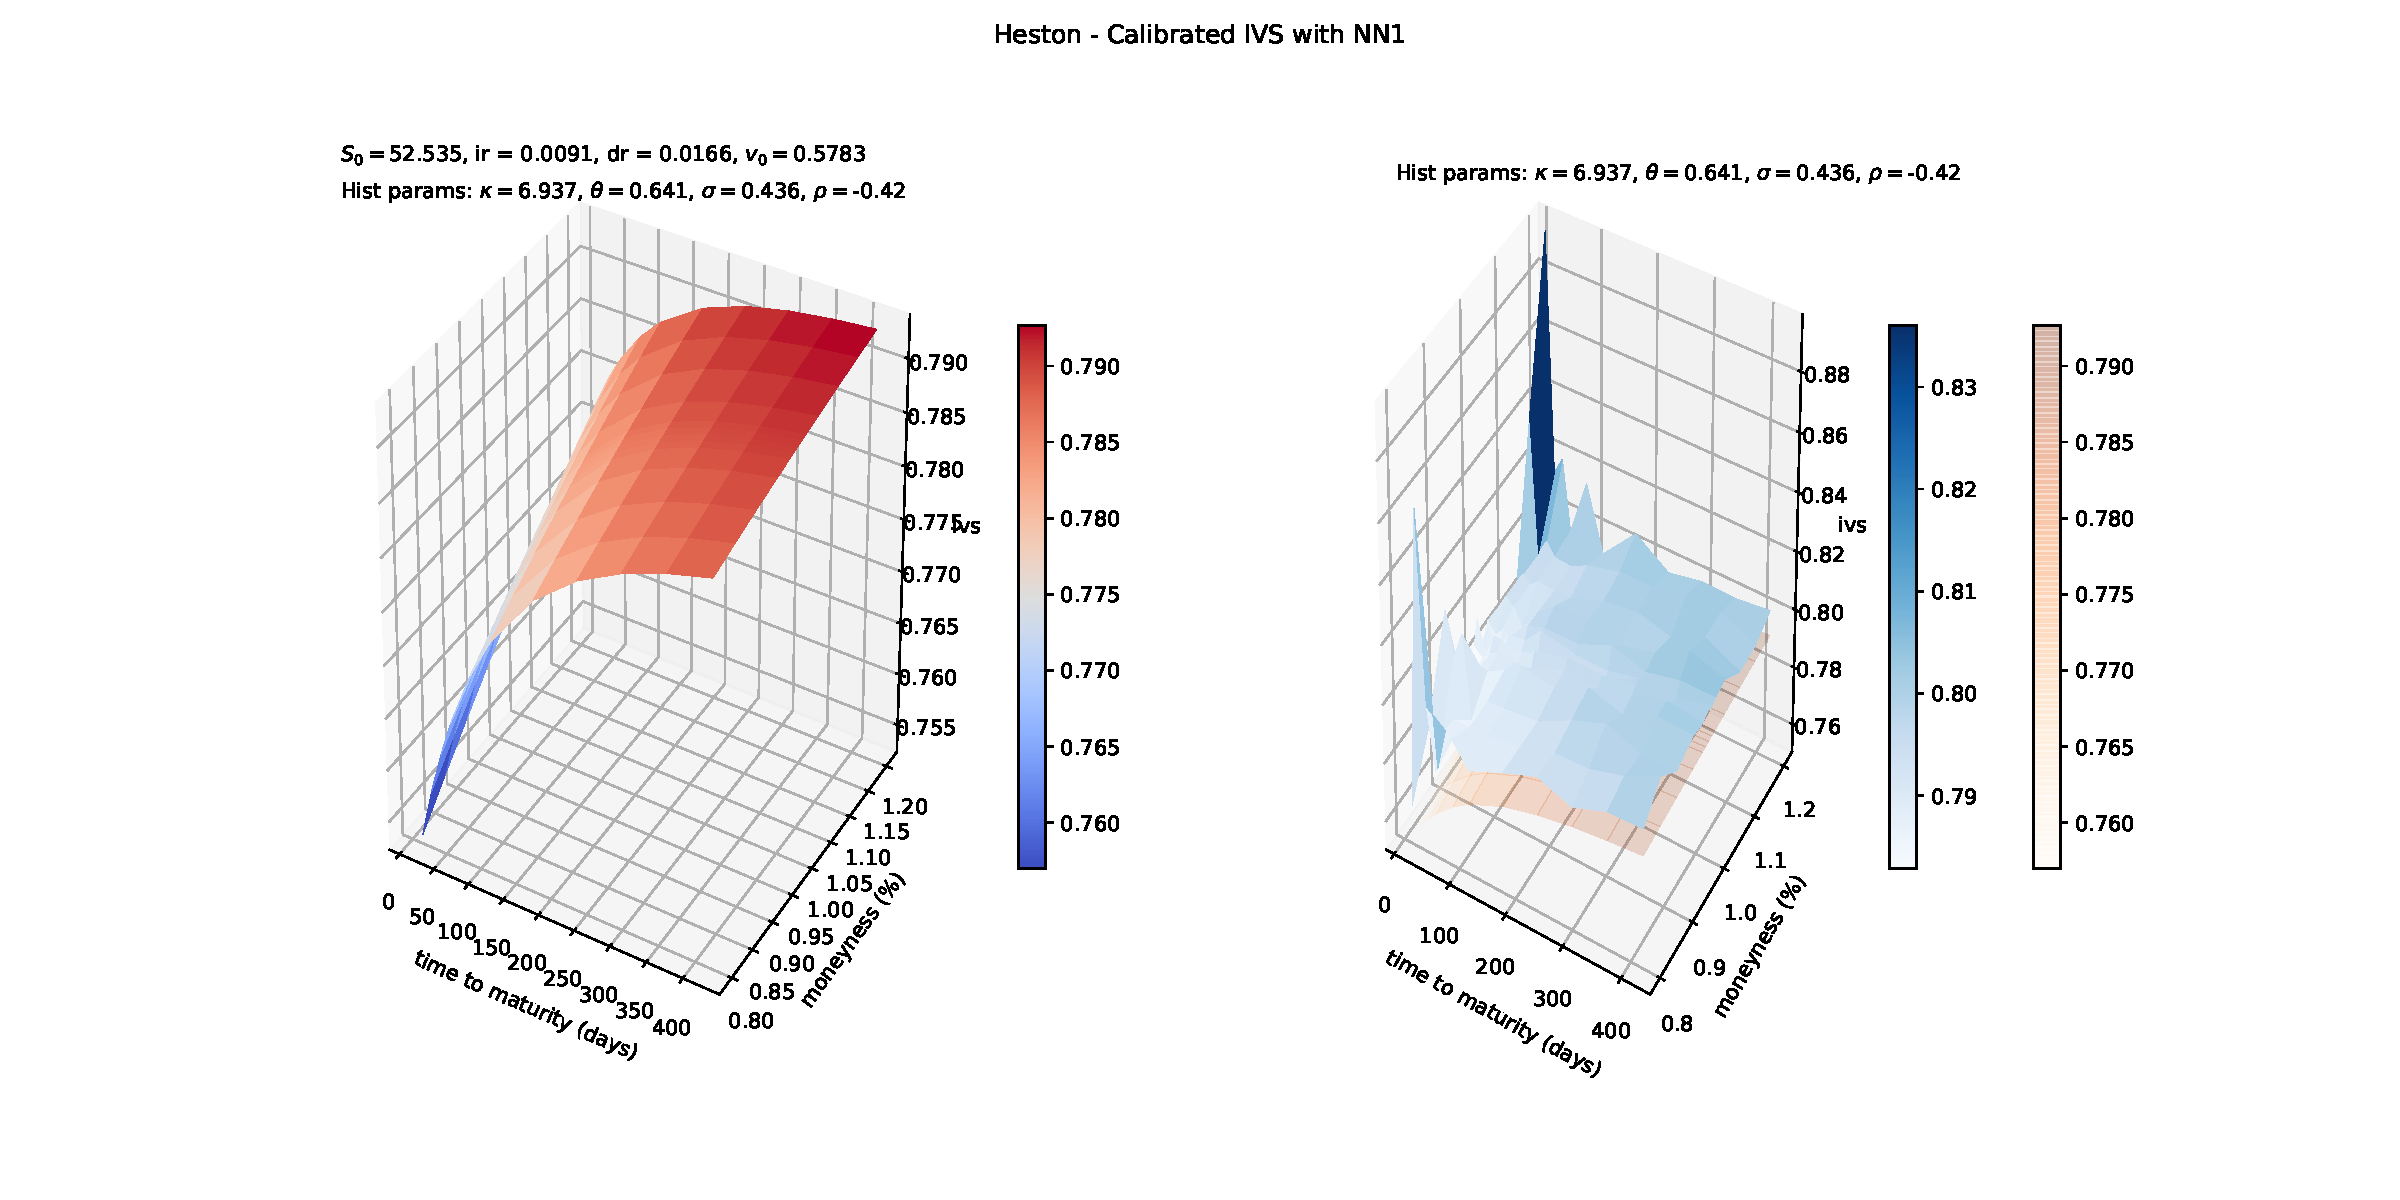
\includegraphics[width=\textwidth]{fig/impvolsurf_0}
	\end{minipage}
	\begin{minipage}{0.49\textwidth}
		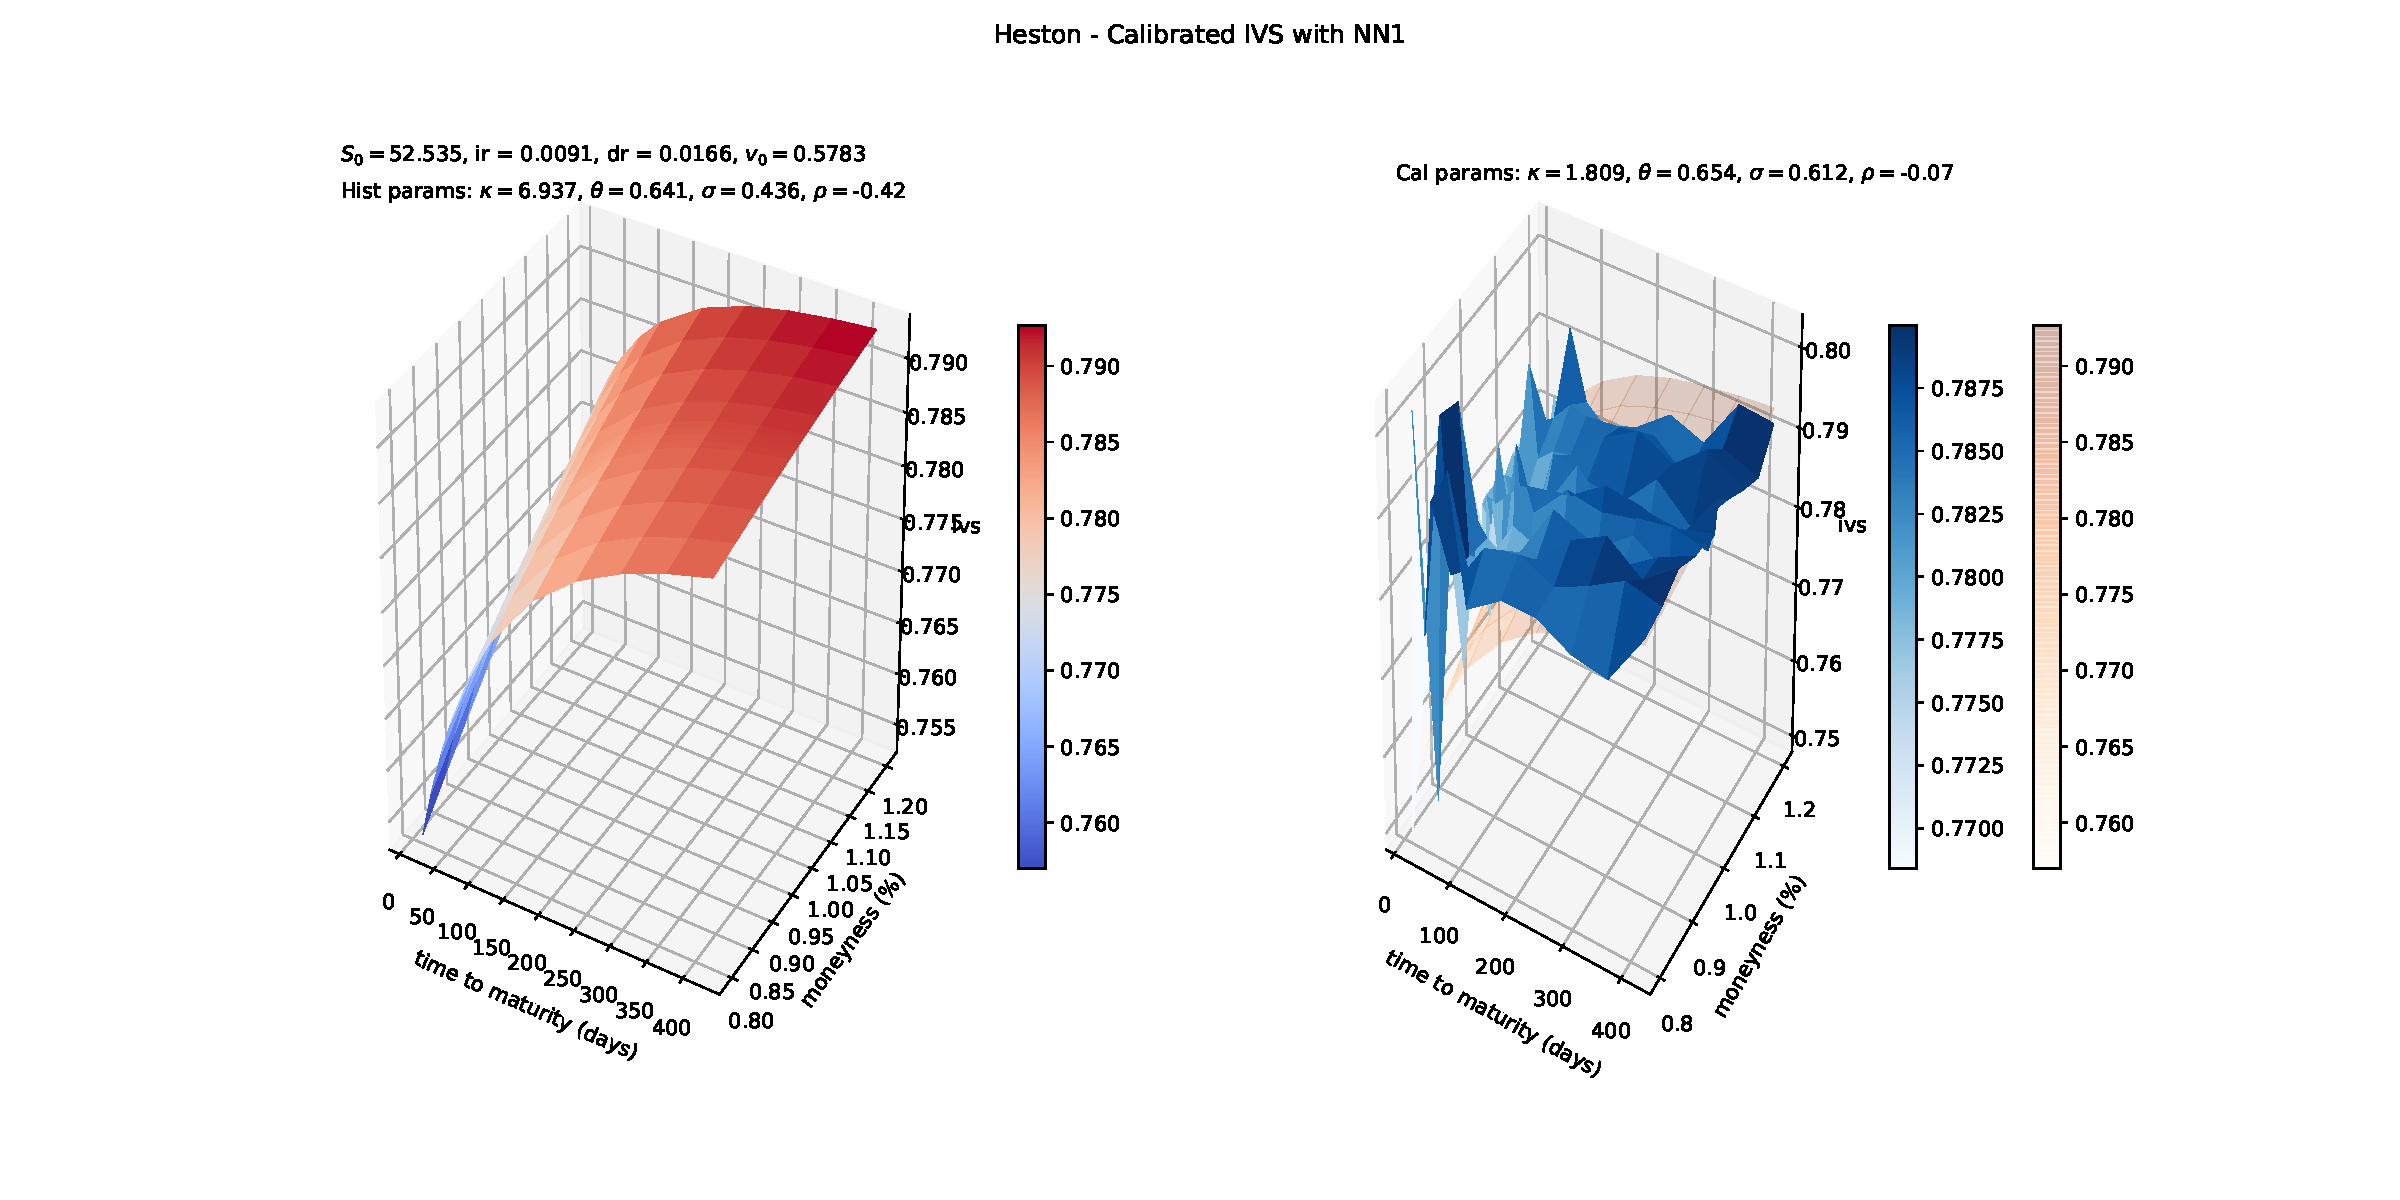
\includegraphics[width=\textwidth]{fig/impvolsurf_calibrated_0}
	\end{minipage}
	\begin{minipage}{0.49\textwidth}
		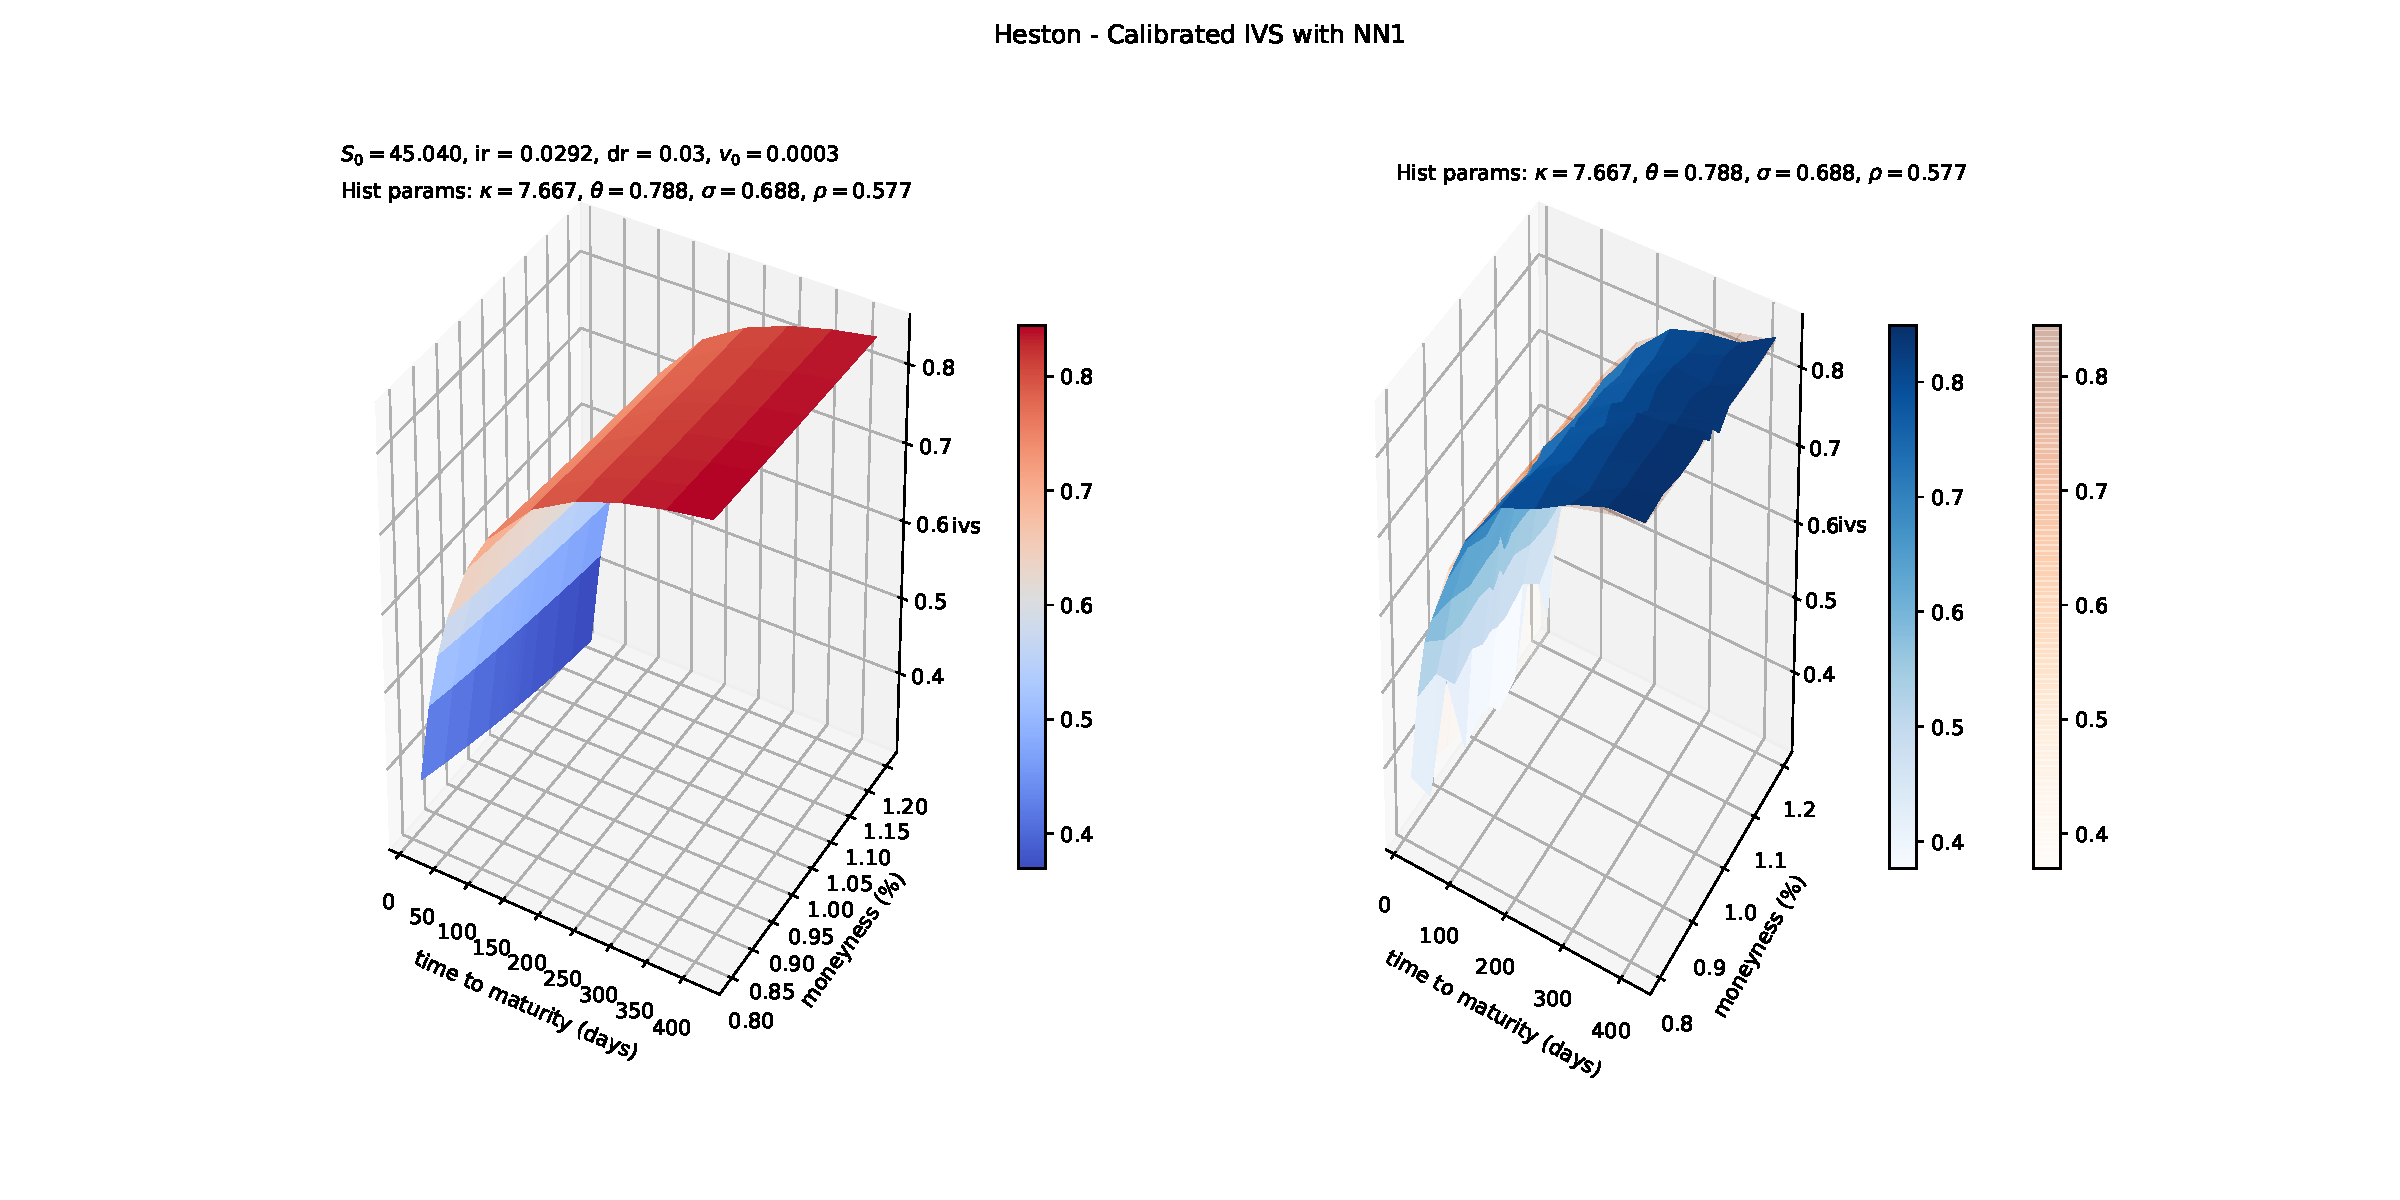
\includegraphics[width=\textwidth]{fig/impvolsurf_1}
	\end{minipage}
	\begin{minipage}{0.49\textwidth}
		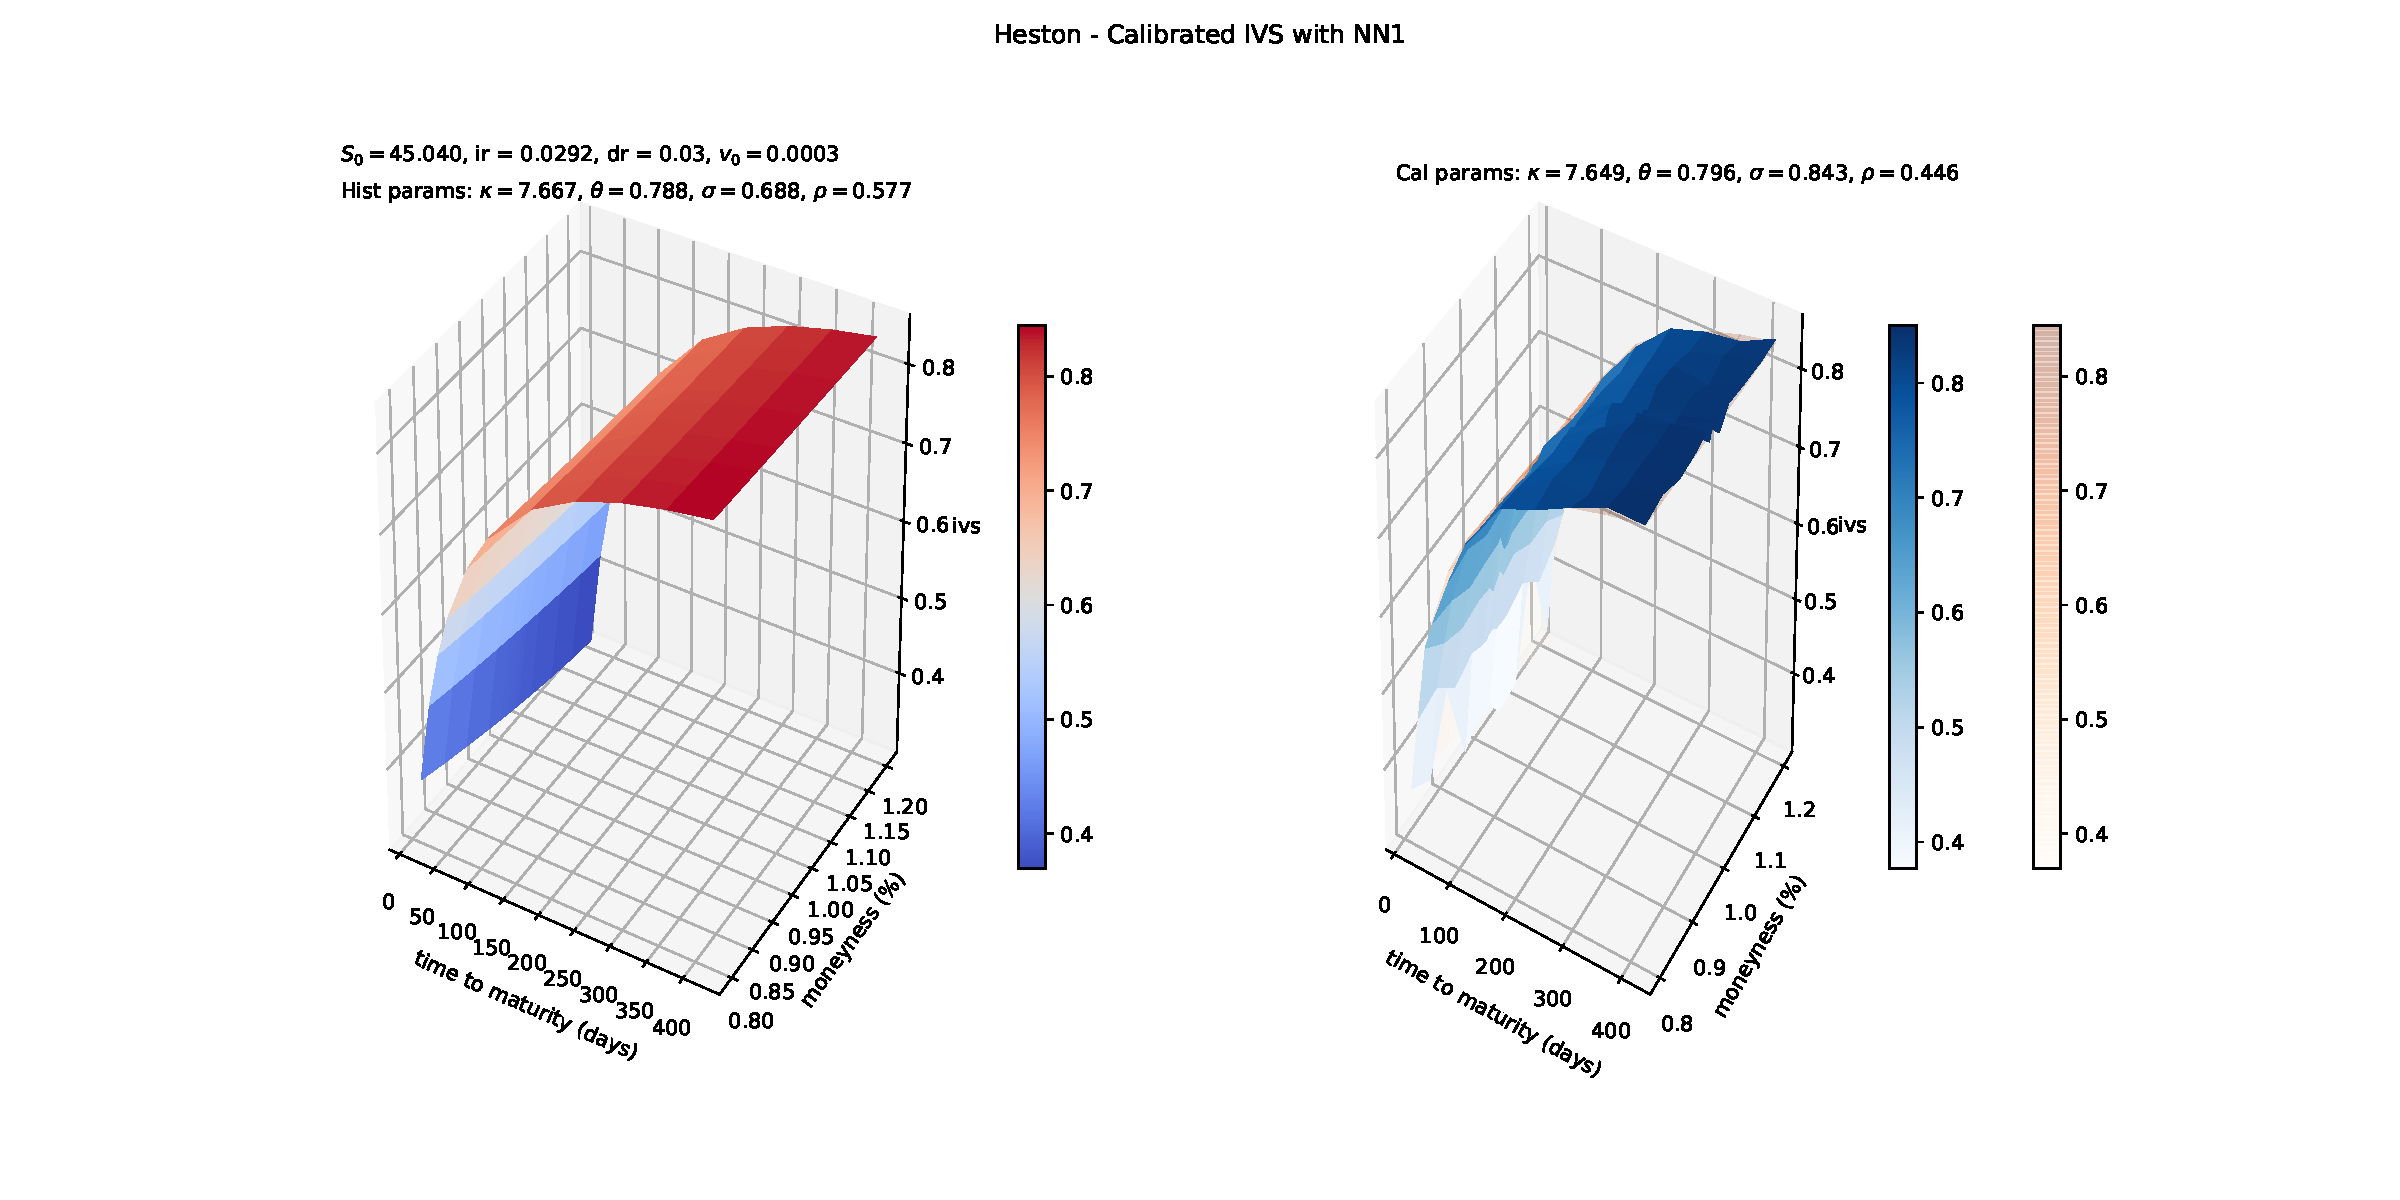
\includegraphics[width=\textwidth]{fig/impvolsurf_calibrated_1}
	\end{minipage}
	\begin{minipage}{0.49\textwidth}
		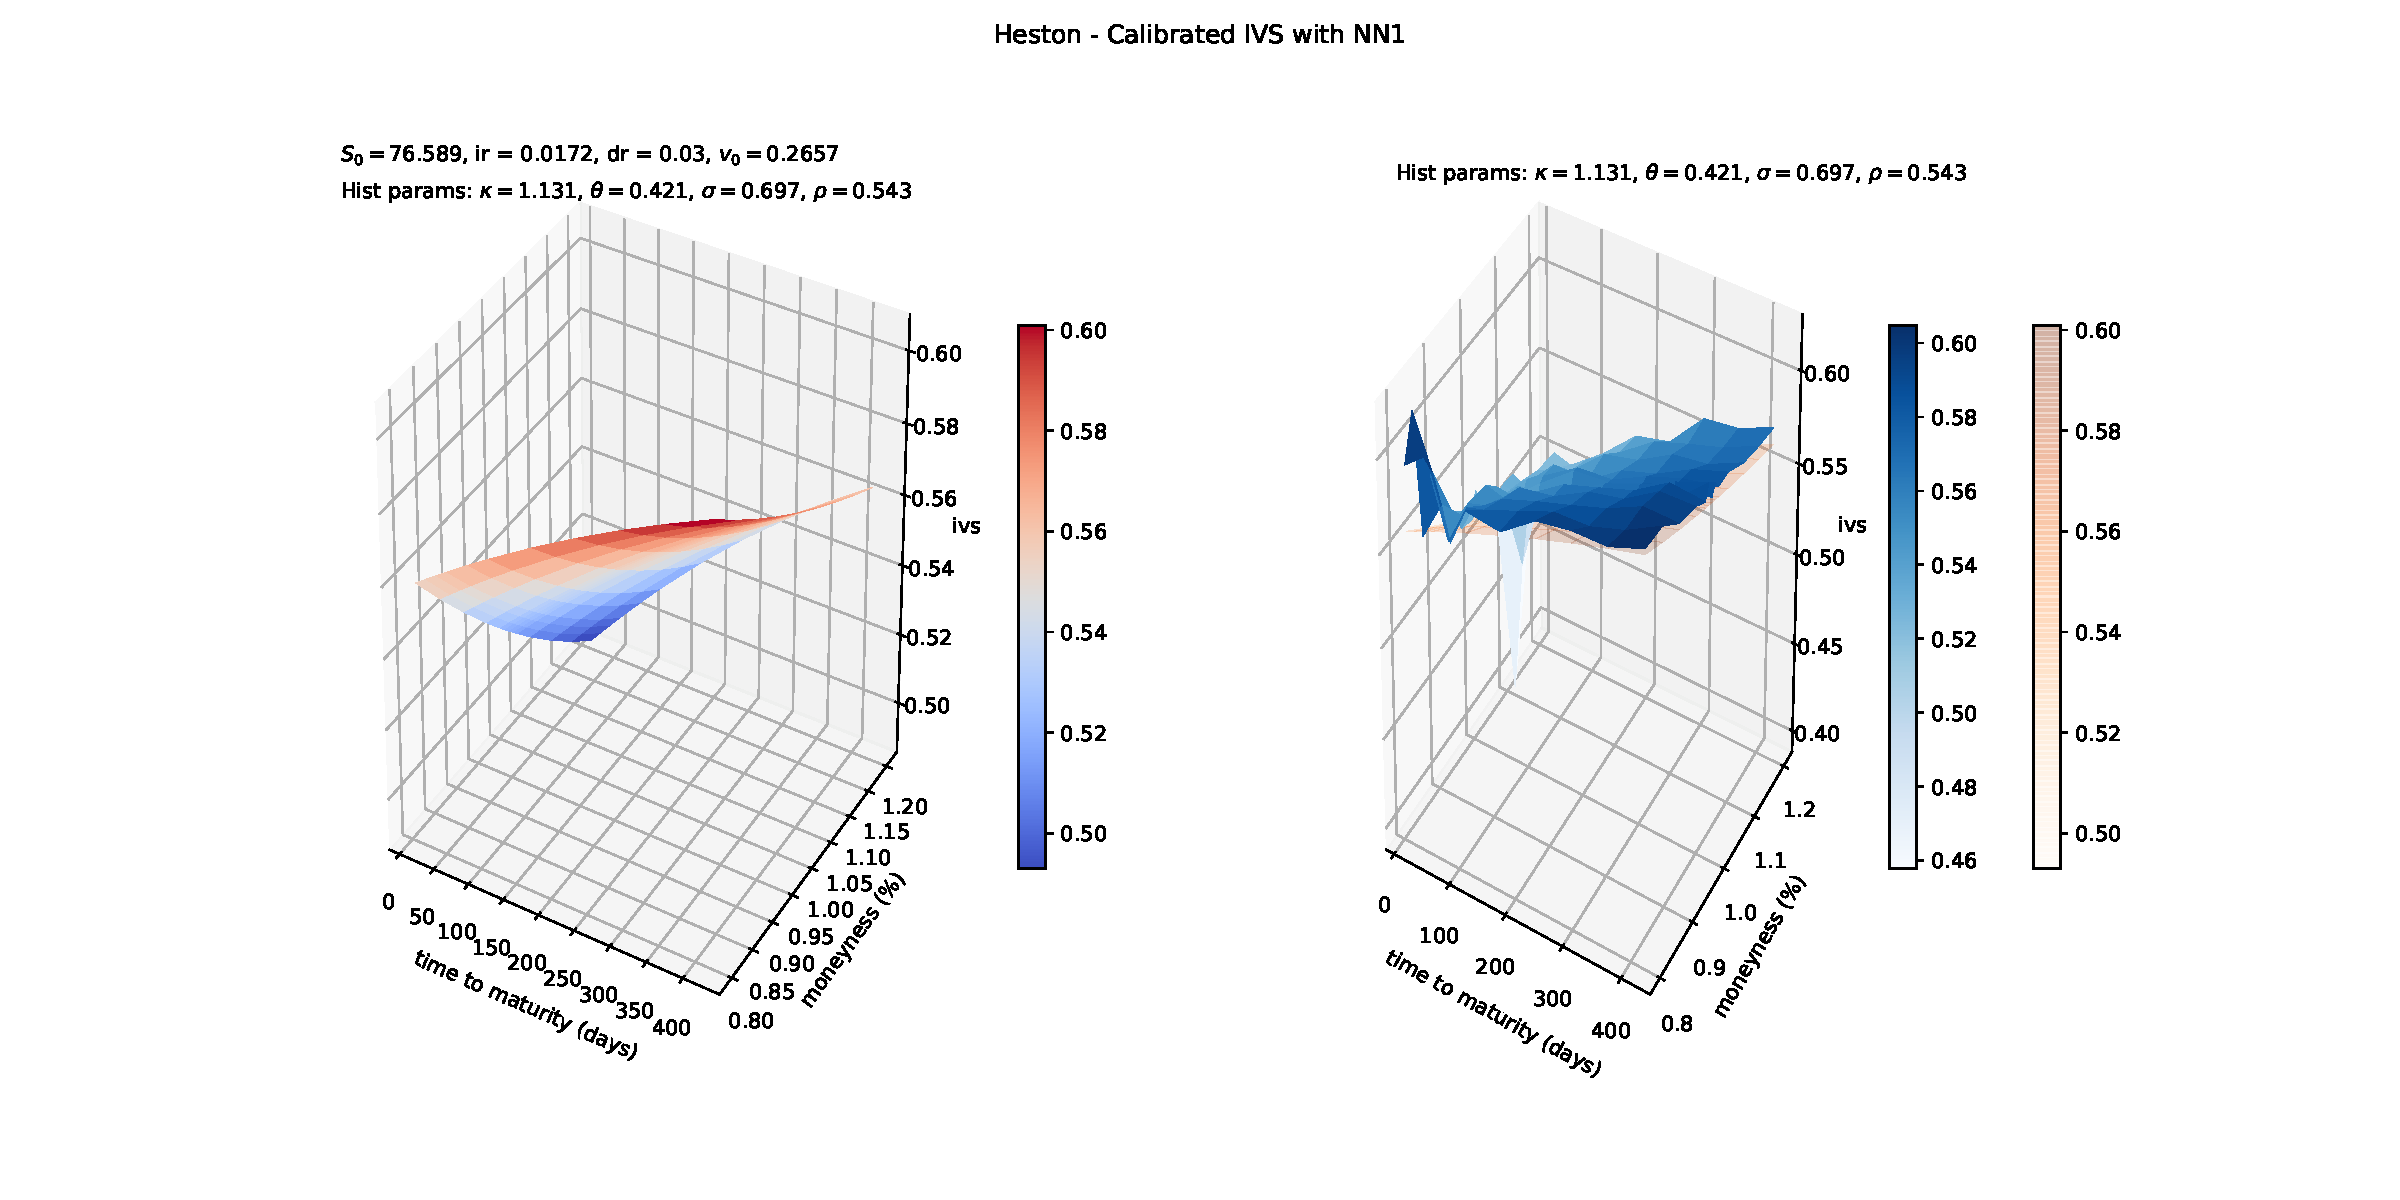
\includegraphics[width=\textwidth]{fig/impvolsurf_2}
	\end{minipage}
	\begin{minipage}{0.49\textwidth}
		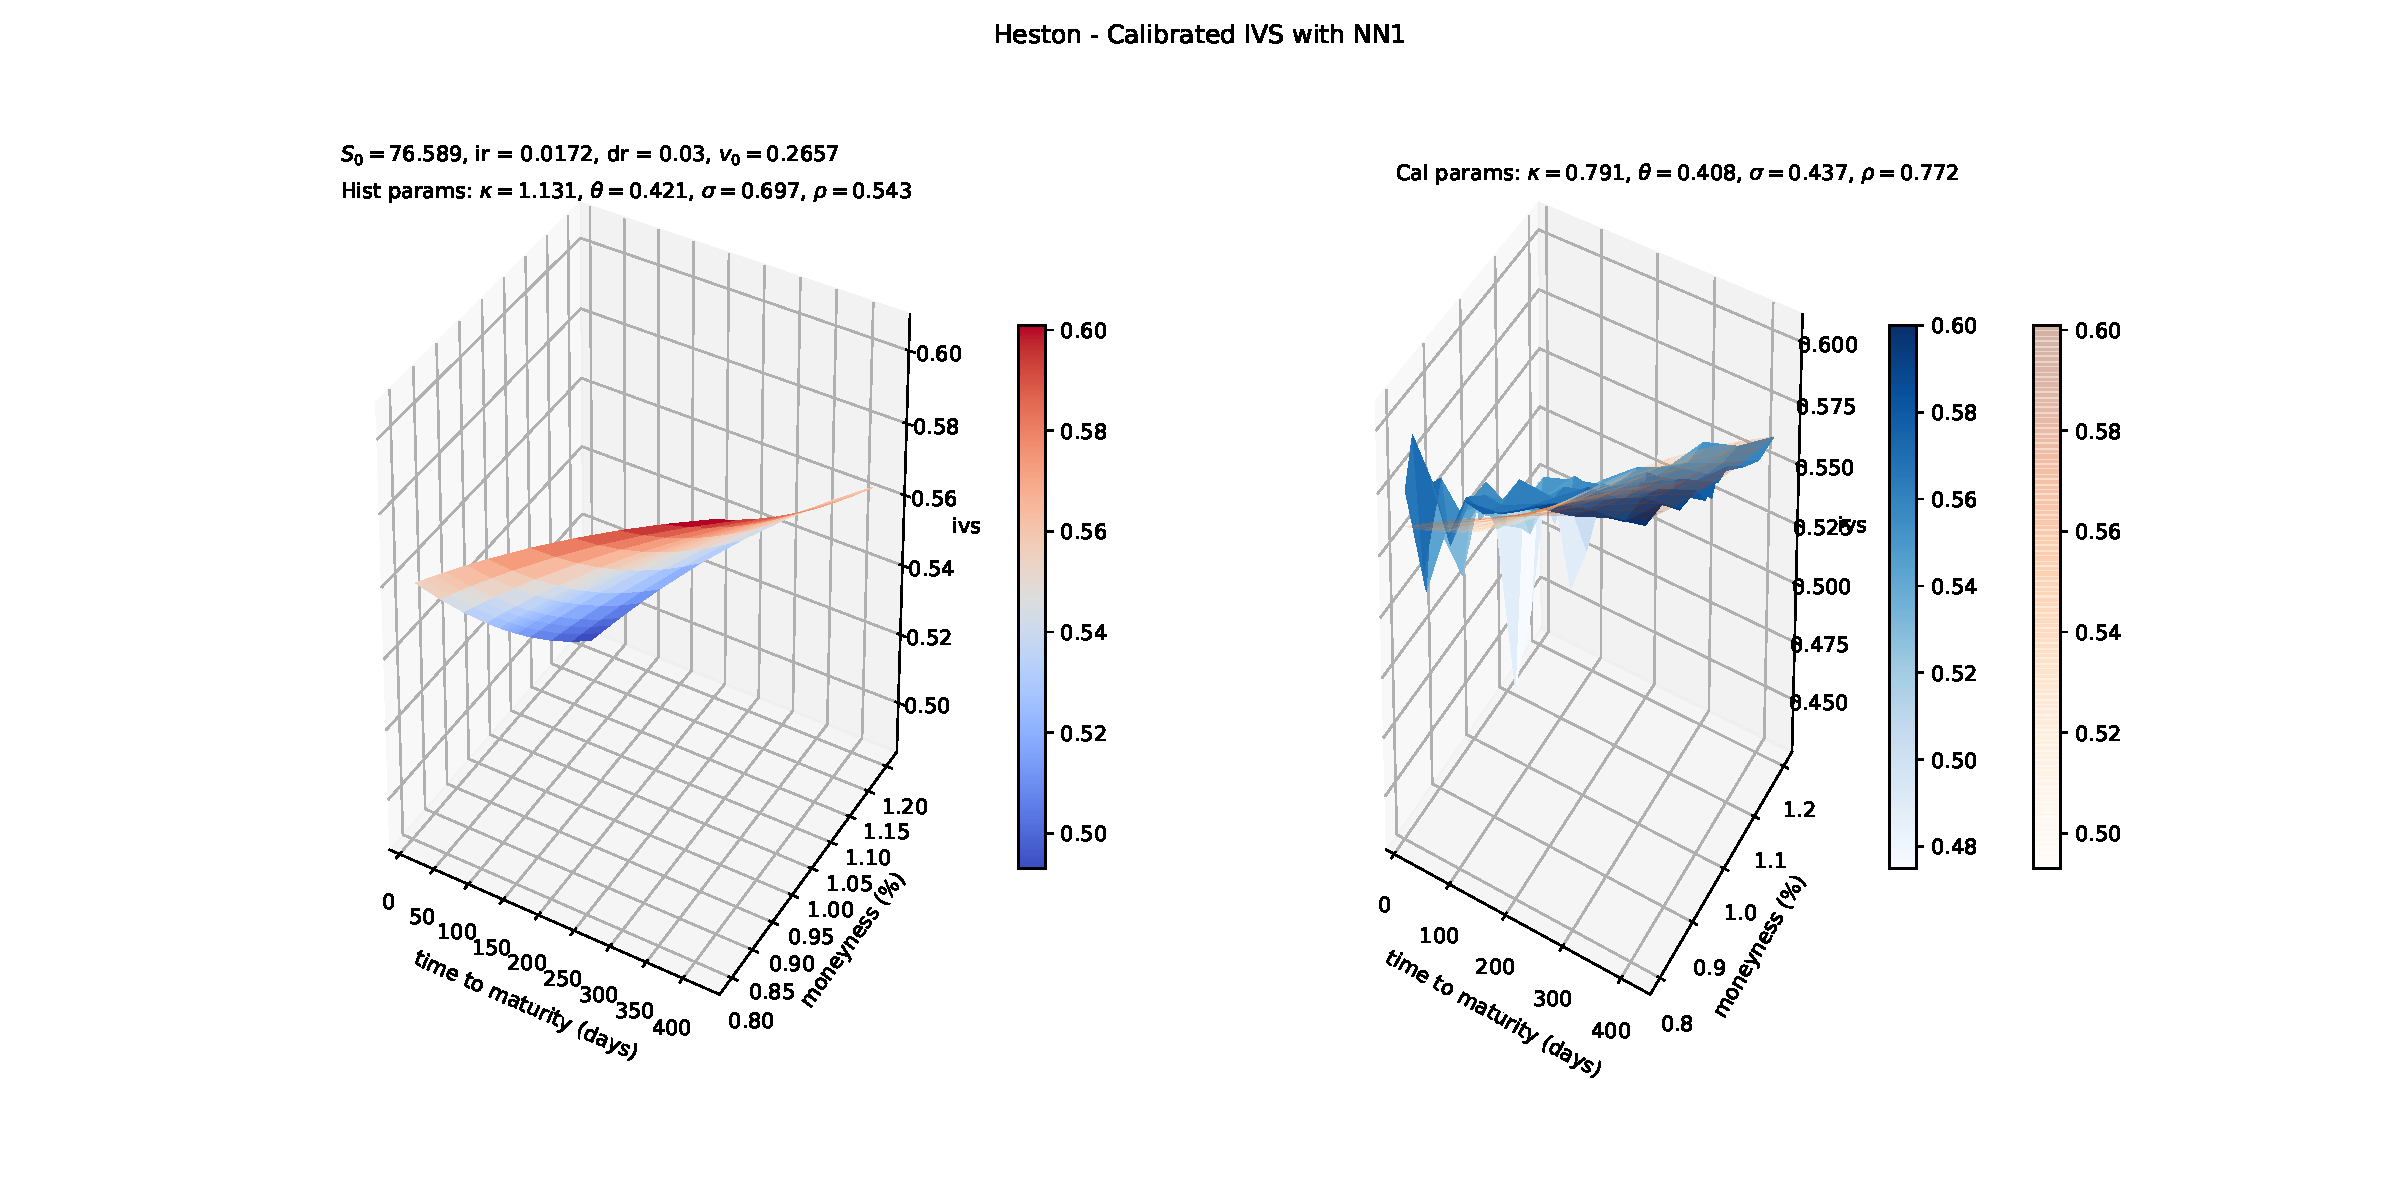
\includegraphics[width=\textwidth]{fig/impvolsurf_calibrated_2}
	\end{minipage}
	\begin{minipage}{0.49\textwidth}
		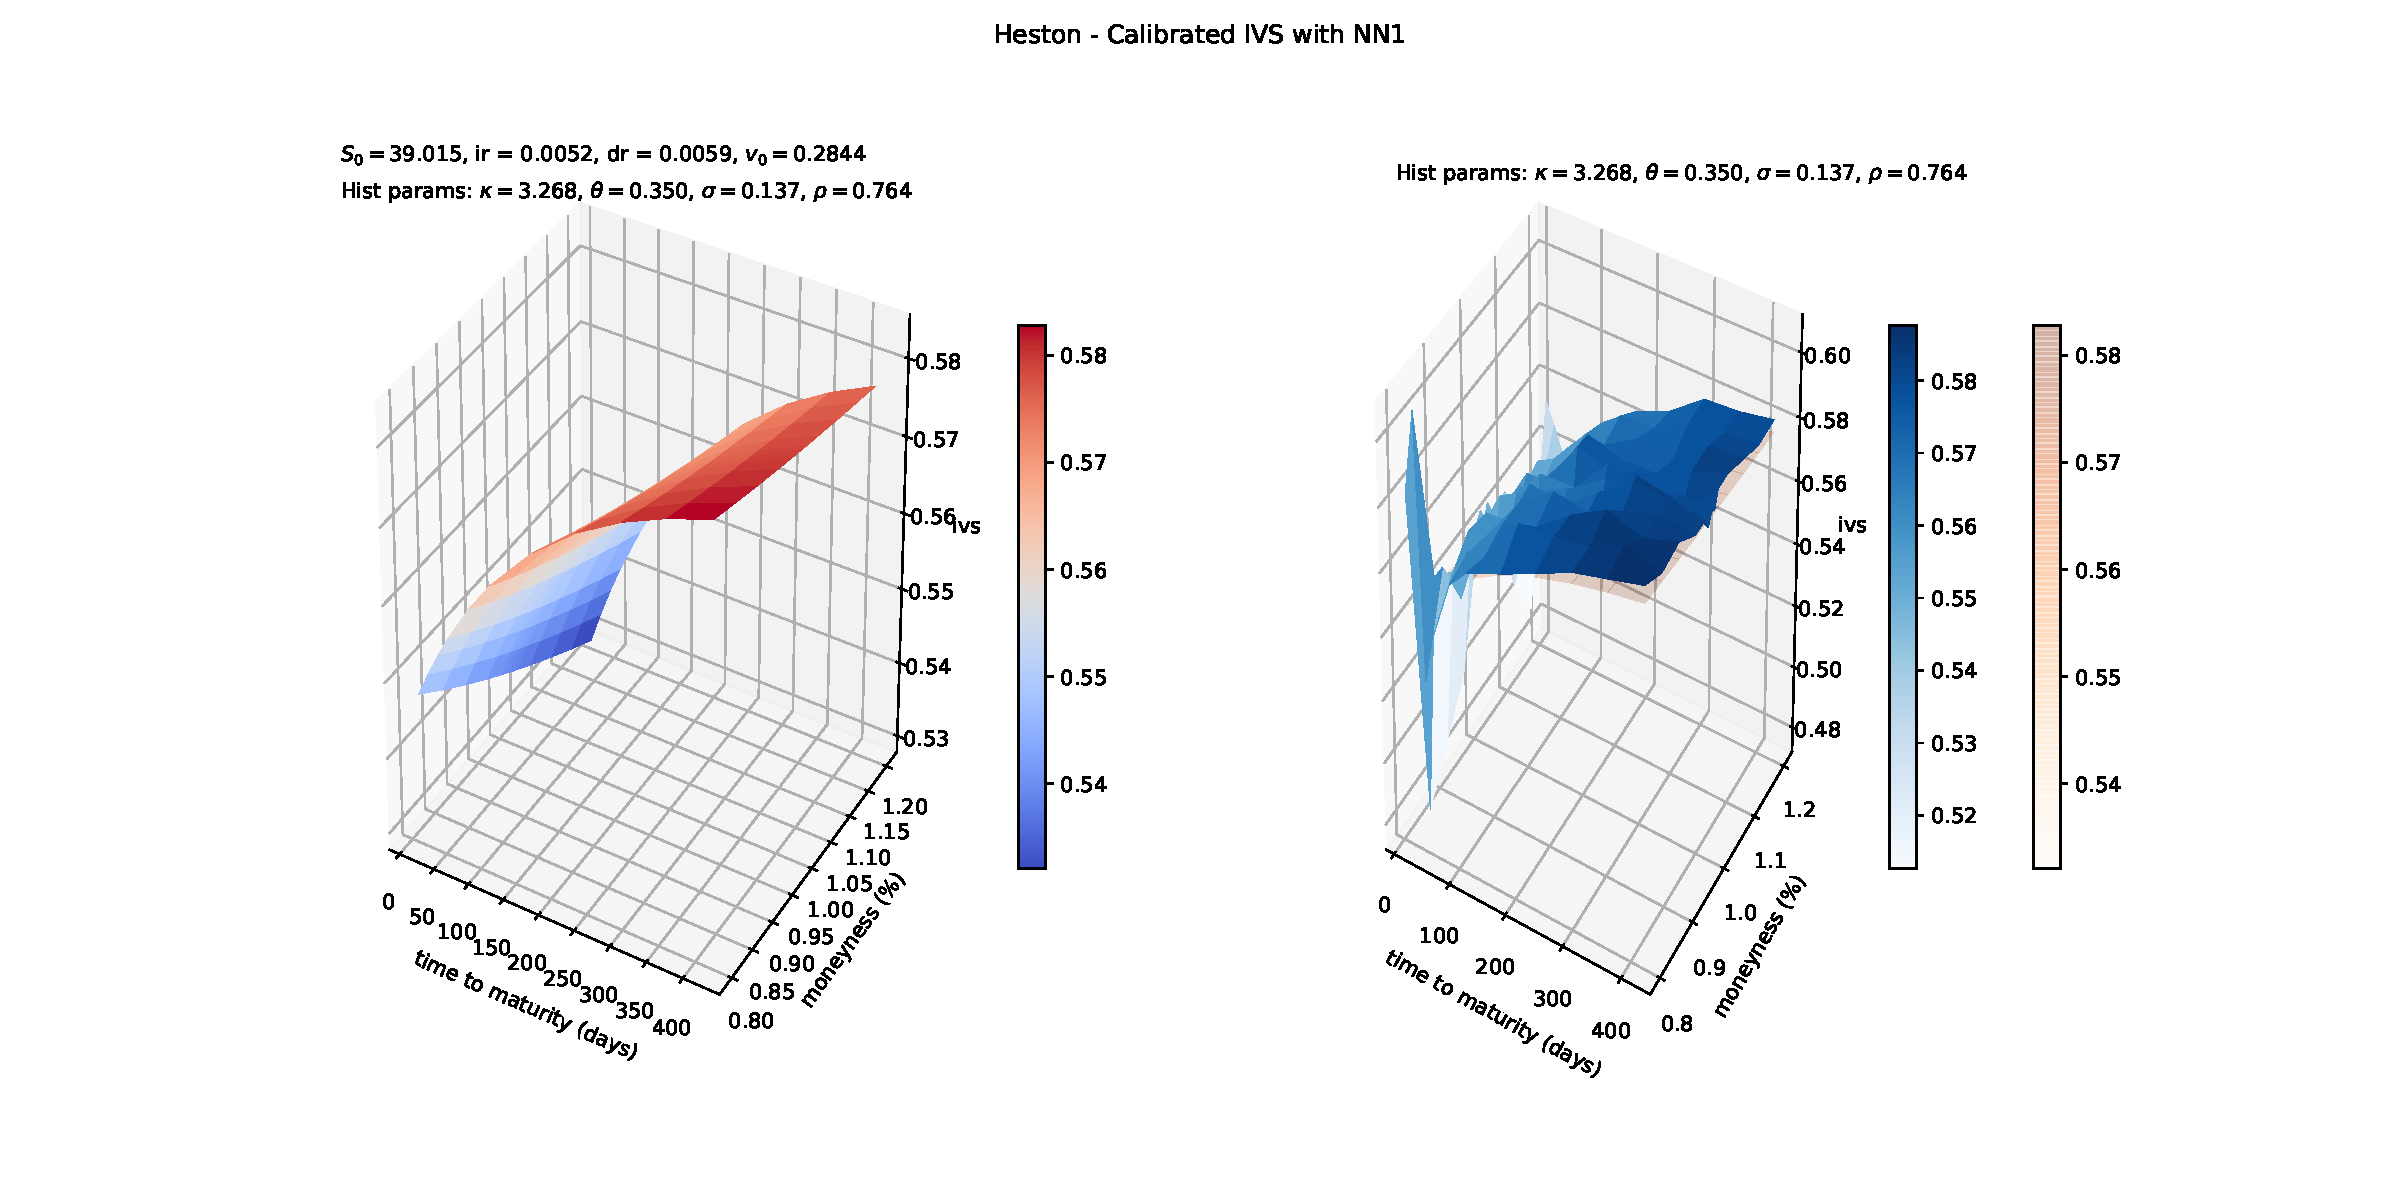
\includegraphics[width=\textwidth]{fig/impvolsurf_3}
	\end{minipage}
	\begin{minipage}{0.49\textwidth}
		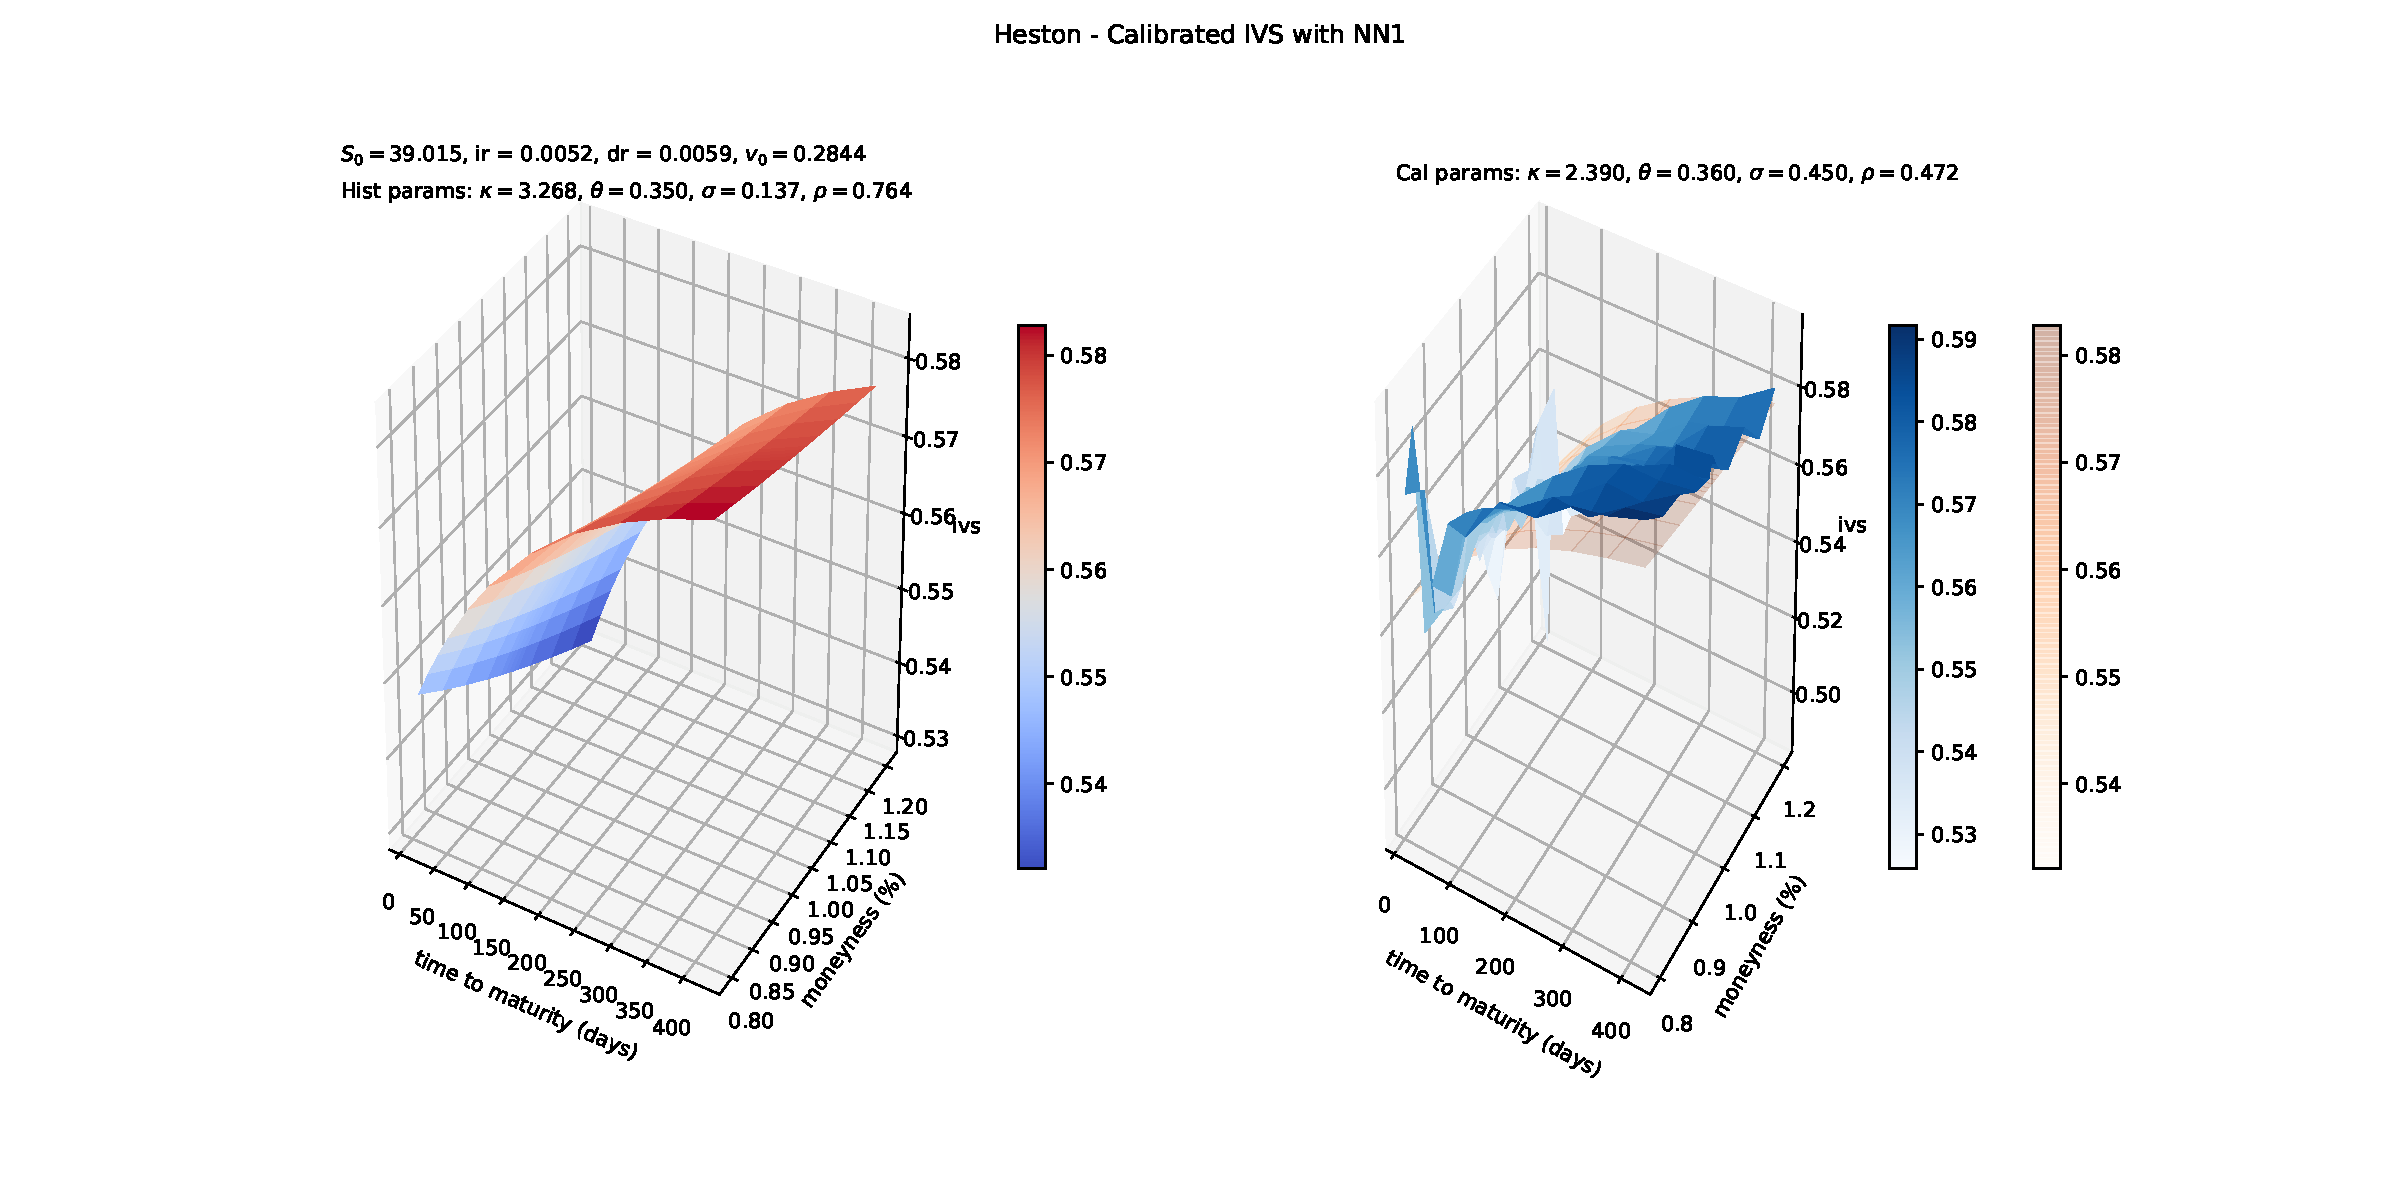
\includegraphics[width=\textwidth]{fig/impvolsurf_calibrated_3}
	\end{minipage}
	\begin{minipage}{0.49\textwidth}
		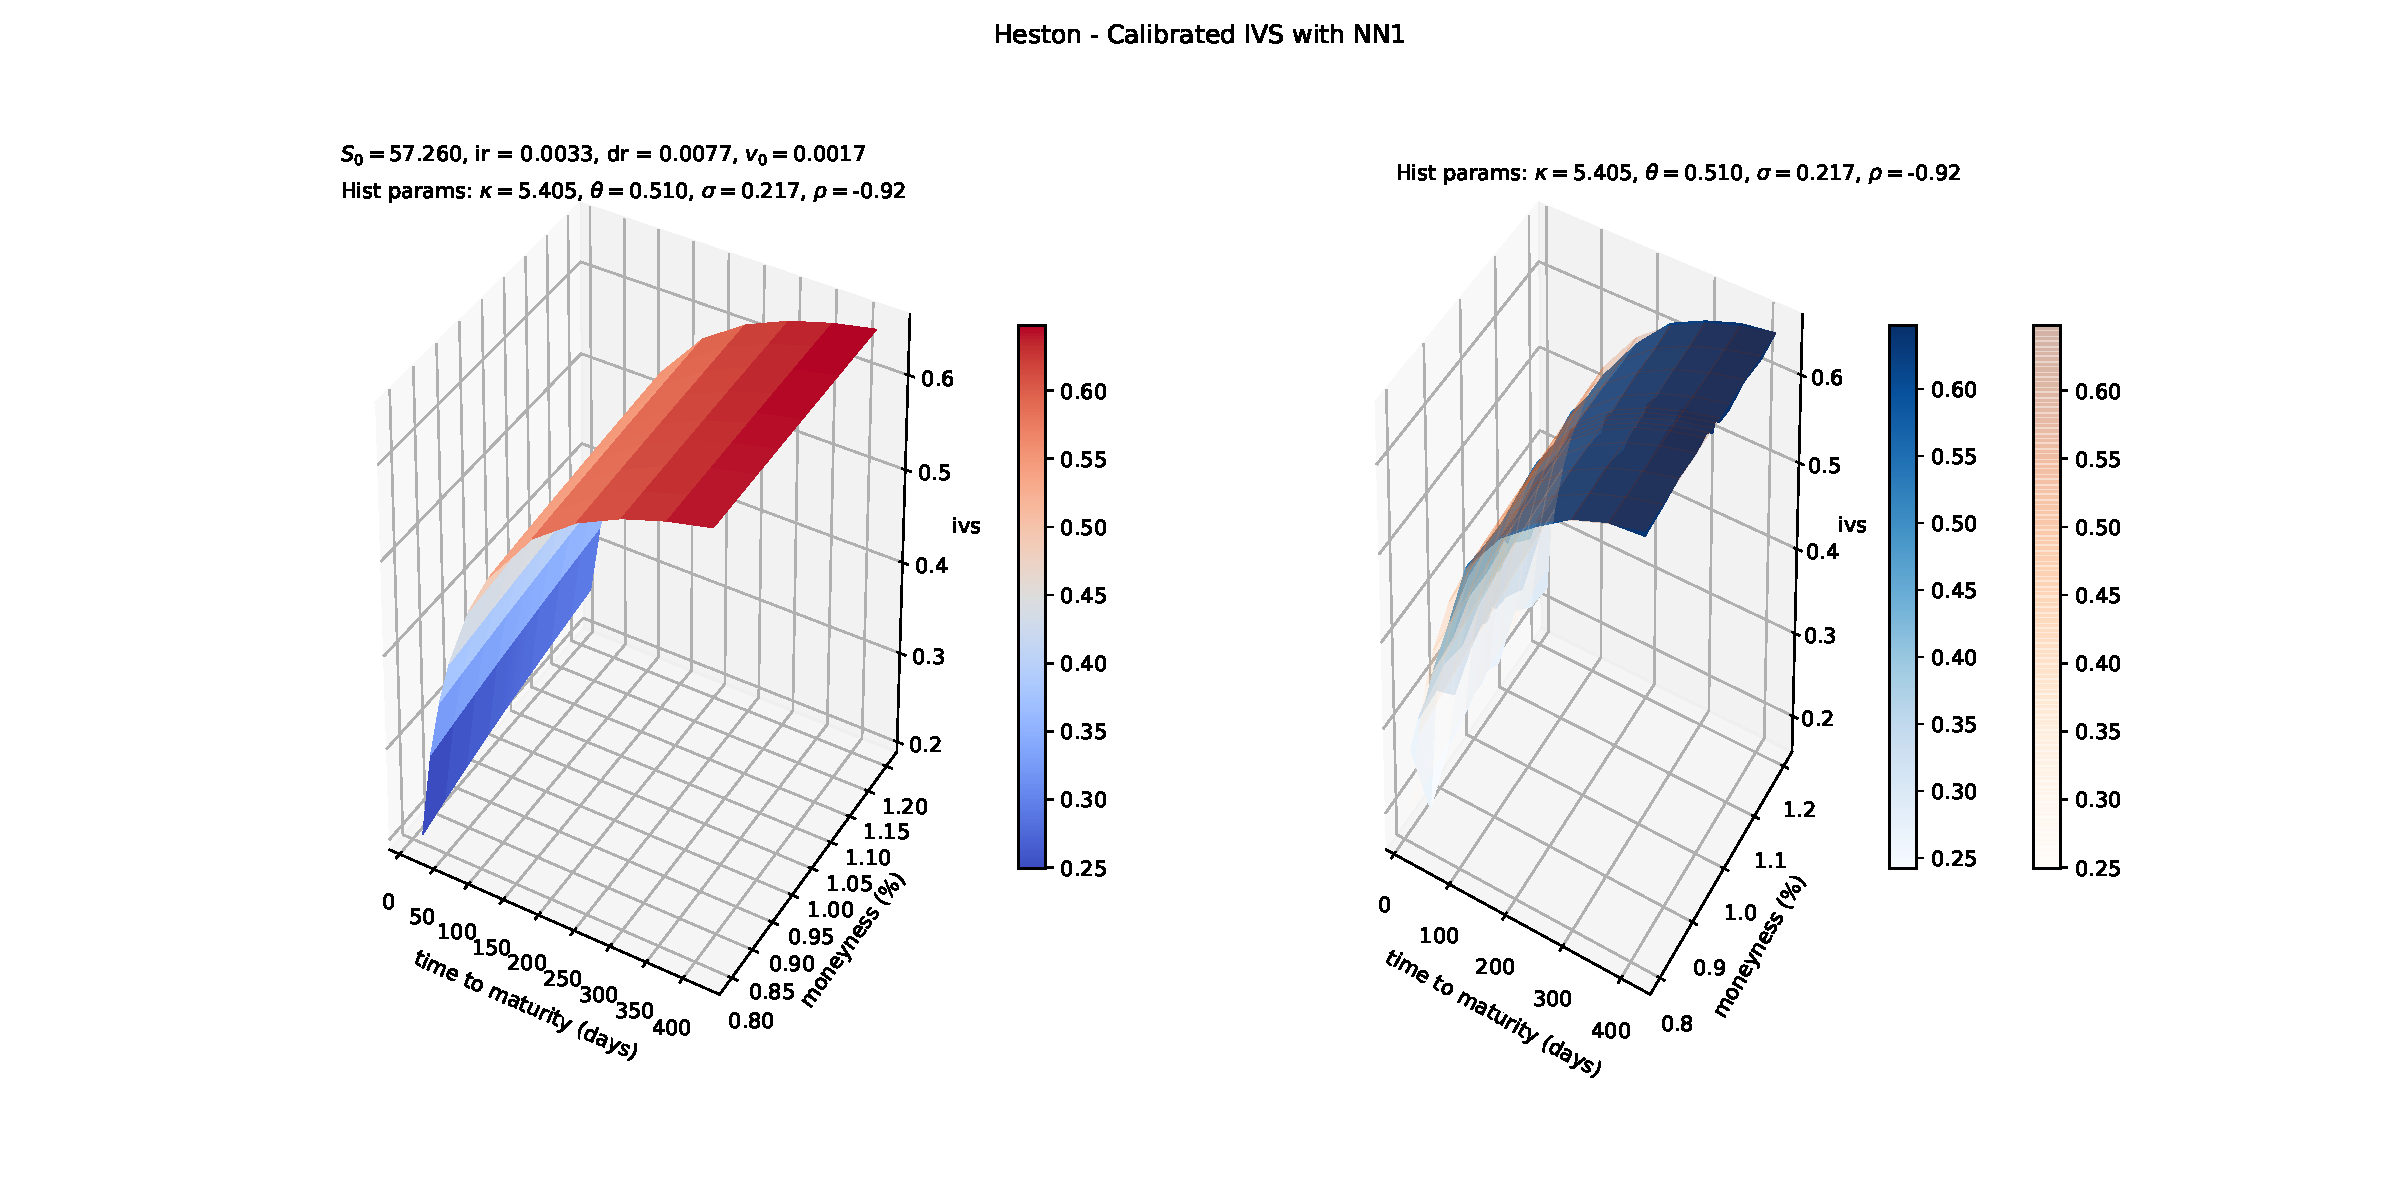
\includegraphics[width=\textwidth]{fig/impvolsurf_4}
	\end{minipage}
	\begin{minipage}{0.49\textwidth}
		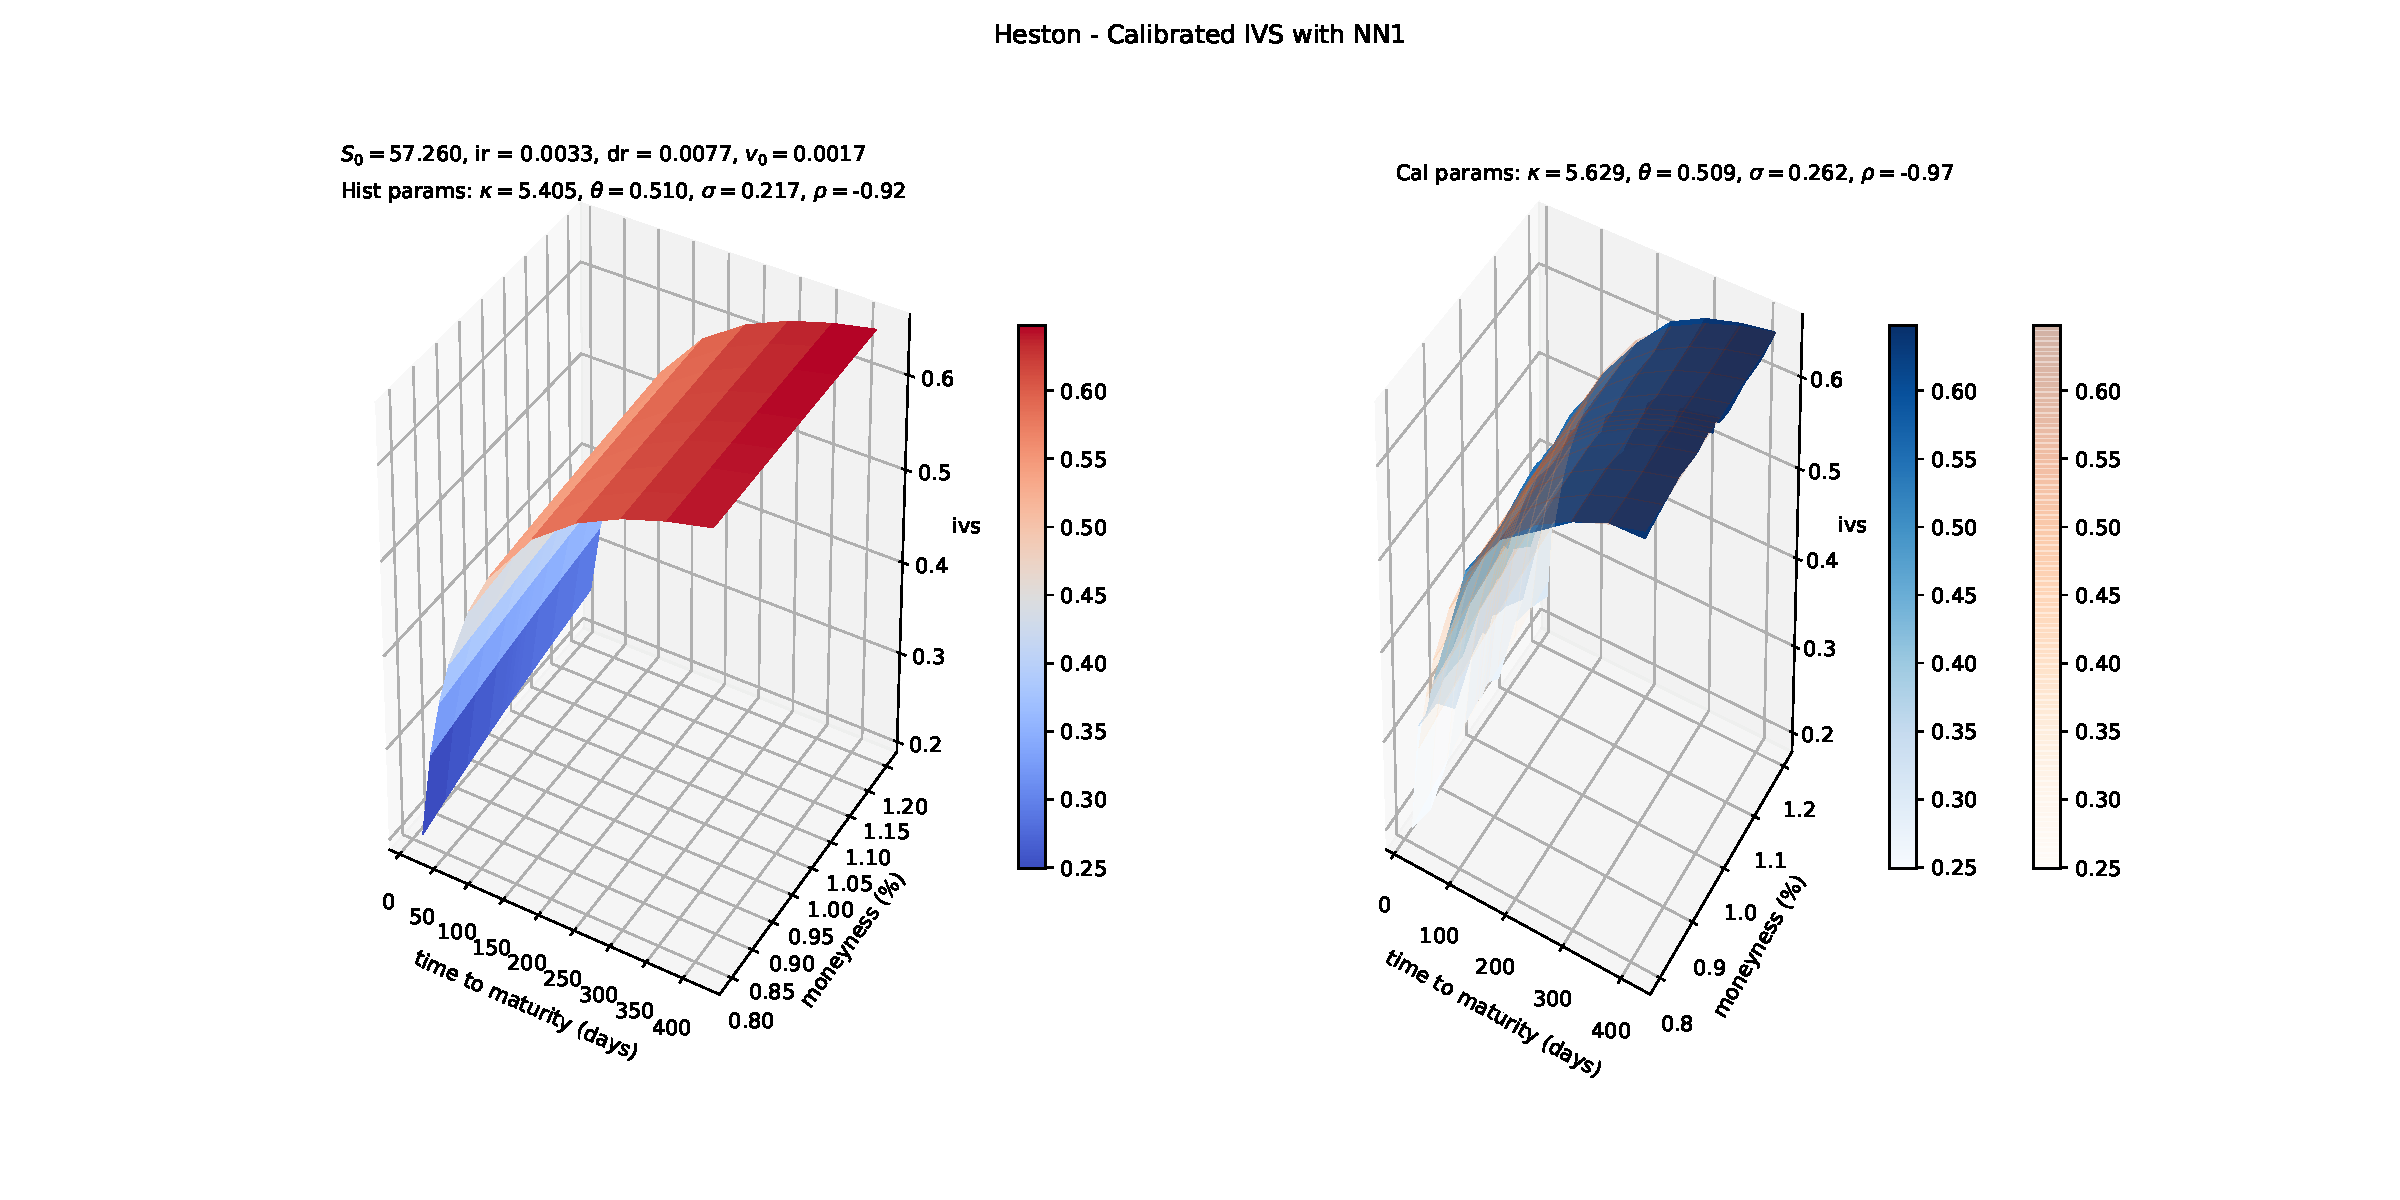
\includegraphics[width=\textwidth]{fig/impvolsurf_calibrated_4}
	\end{minipage}
	\caption{Calibration of the stochastic volatility part. The left column shows implied volatility surfaces for the historical parameters (indicated in each subplot) generated by the Heston model (left) vs. the surface generated via the neural network (right) for the same parameter choice. The right column shows a comparison of both implied volatility surfaces after calibration. In the most right subplots the calibrated parameters for each day are shown.}
	\label{fig:calibration_svpart}
\end{figure}

\section{Calibration of local volatility}\label{sec:calibLV}

In the second notebook \texttt{SLV-calib-local.ipynb}, we first compare the price surfaces of the true parameters against the price surfaces of the calibrated parameters (following the calibration routine of the stochastic volatility implemented in the first notebook) generated by the network scheme of the second notebook with trivial leverage function $L(t,S_t)=1$ (i.e. before training) (again for each of the five days). Figure \ref{fig:pricesurf_comparison_untrained} shows both surfaces of European call option prices on a grid of strikes $K$ and maturities $T$. The prices from the network are calculated in by averaging $10^4$ paths (in total batch mode). As one can see, the true surface are qualitatively well reproduced which certifies the suitability of the employed scheme to calibrate the stochastic part of the SLV-model in \texttt{SLV-calib-stochastic.ipynb}. However, the difference plots (Fig. \ref{fig:pricesurf_comparison_untrained}, right panel) transparently show the discrepancy of the calibrated model from the true data. On this difference we try to improve in the following by the calibration of the stochastic part, i.e. the direct learning of the leverage function.


\begin{figure}
	\begin{minipage}[Ausrichtung]{0.329\textwidth}
		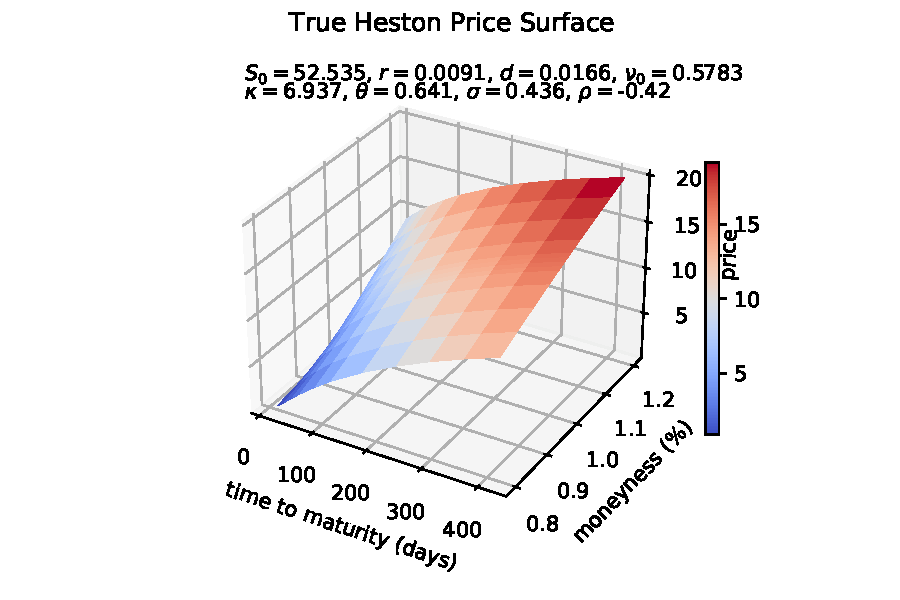
\includegraphics[width=\textwidth]{fig/Psurf_orginal_2017-01-01}
	\end{minipage}
	\begin{minipage}[Ausrichtung]{0.329\textwidth}
		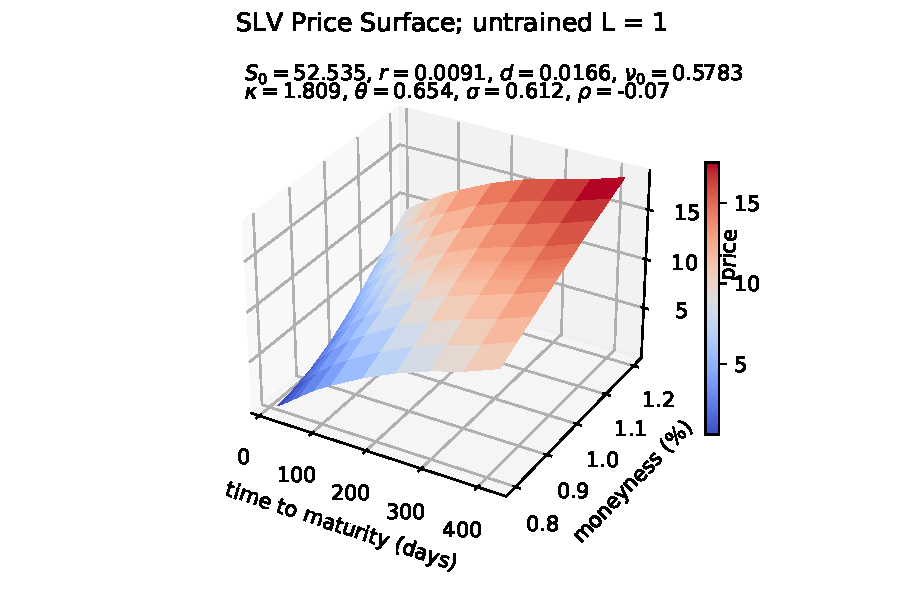
\includegraphics[width=\textwidth]{fig/Psurf_untrained_2017-01-01}
	\end{minipage}
	\begin{minipage}[Ausrichtung]{0.329\textwidth}
		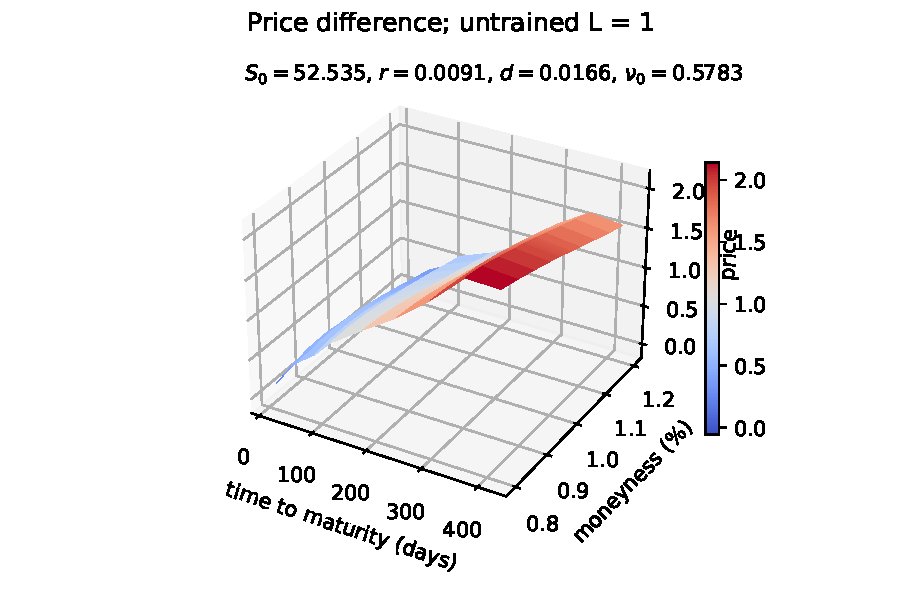
\includegraphics[width=\textwidth]{fig/Psurf_untrained_diff_2017-01-01_rec_3lay_seed1}
	\end{minipage}
	\begin{minipage}[Ausrichtung]{0.329\textwidth}
		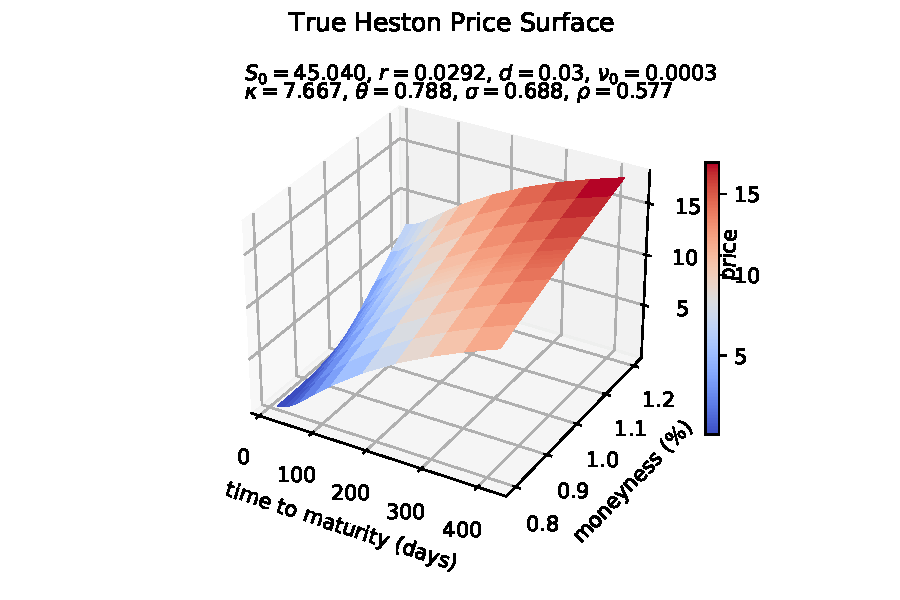
\includegraphics[width=\textwidth]{fig/Psurf_orginal_2017-01-02}
	\end{minipage}
	\begin{minipage}[Ausrichtung]{0.329\textwidth}
		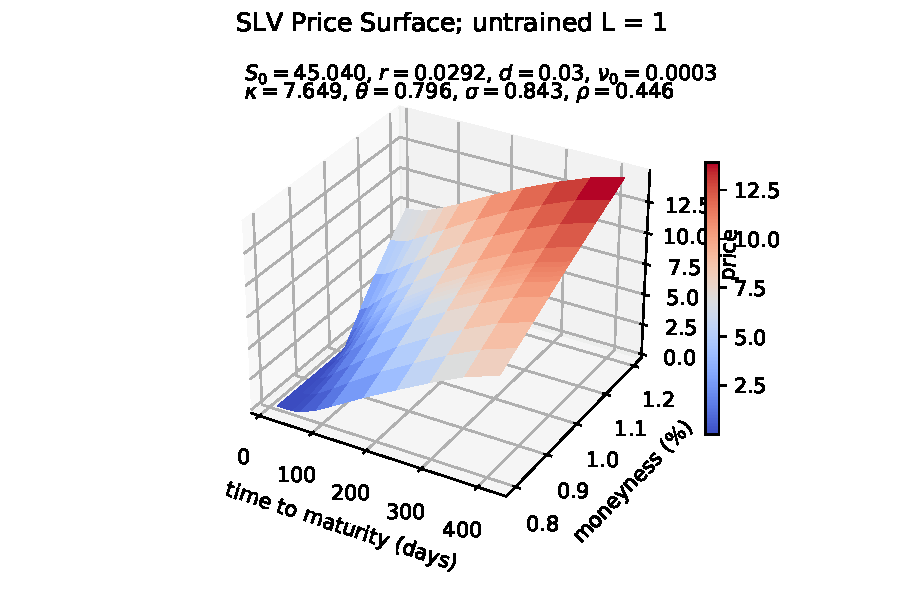
\includegraphics[width=\textwidth]{fig/Psurf_untrained_2017-01-02}
	\end{minipage}
	\begin{minipage}[Ausrichtung]{0.329\textwidth}
		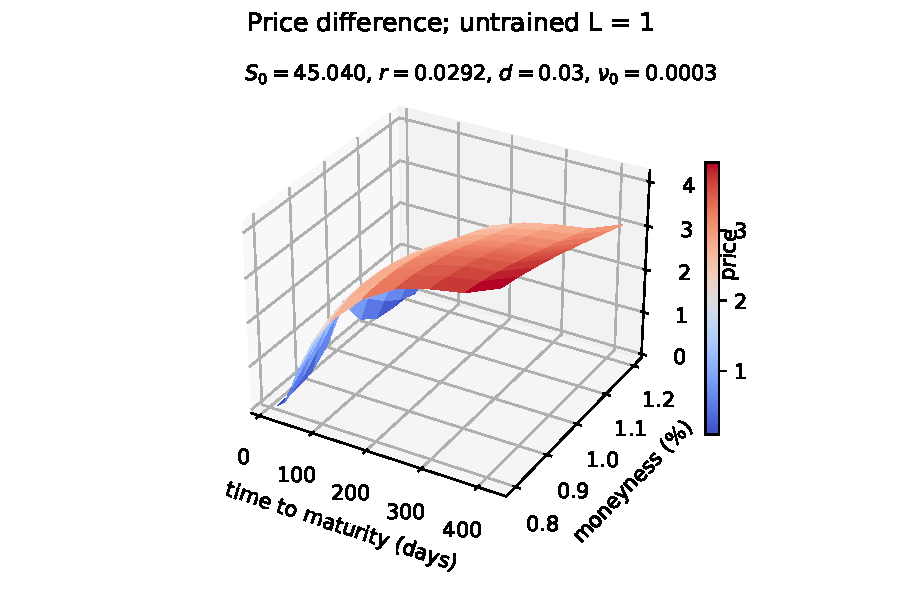
\includegraphics[width=\textwidth]{fig/Psurf_untrained_diff_2017-01-02_rec_3lay_seed1}
	\end{minipage}
	\begin{minipage}[Ausrichtung]{0.329\textwidth}
		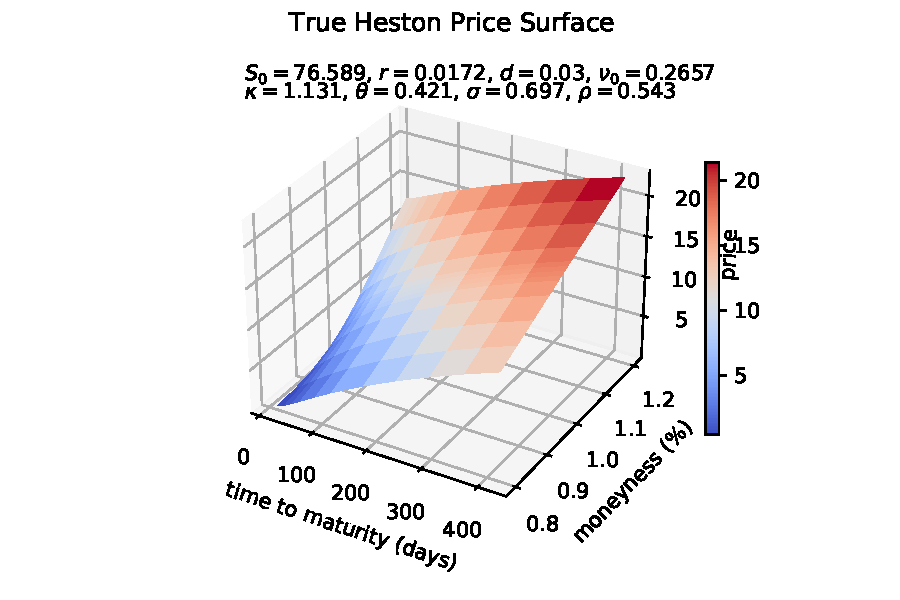
\includegraphics[width=\textwidth]{fig/Psurf_orginal_2017-01-03}
	\end{minipage}
	\begin{minipage}[Ausrichtung]{0.329\textwidth}
		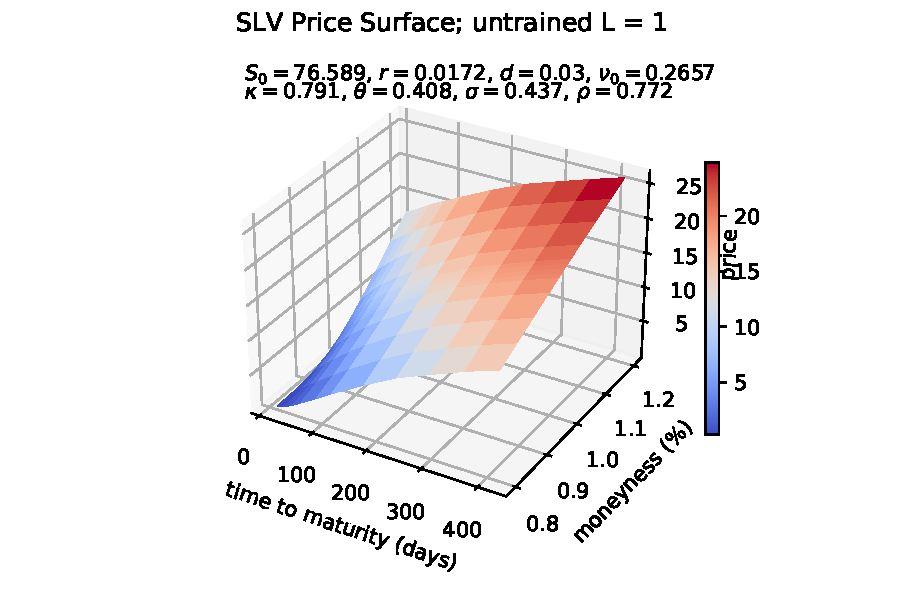
\includegraphics[width=\textwidth]{fig/Psurf_untrained_2017-01-03}
	\end{minipage}
	\begin{minipage}[Ausrichtung]{0.329\textwidth}
		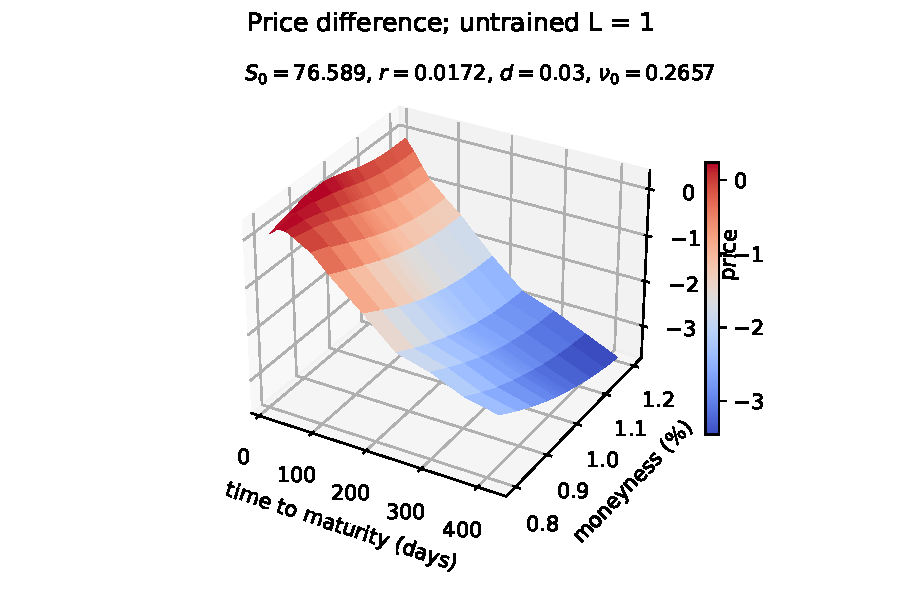
\includegraphics[width=\textwidth]{fig/Psurf_untrained_diff_2017-01-03_rec_3lay_seed1}
	\end{minipage}
	\begin{minipage}[Ausrichtung]{0.329\textwidth}
		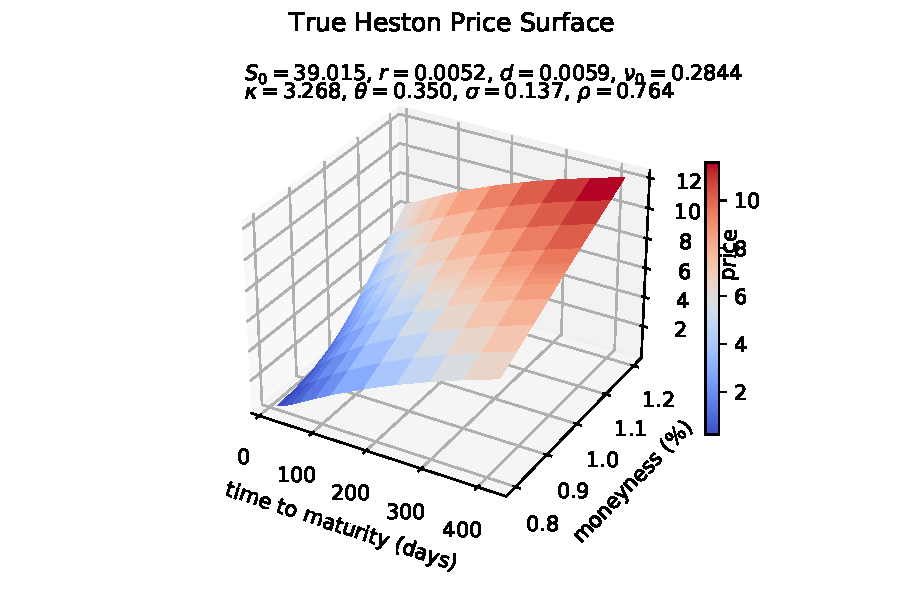
\includegraphics[width=\textwidth]{fig/Psurf_orginal_2017-01-04}
	\end{minipage}
	\begin{minipage}[Ausrichtung]{0.329\textwidth}
		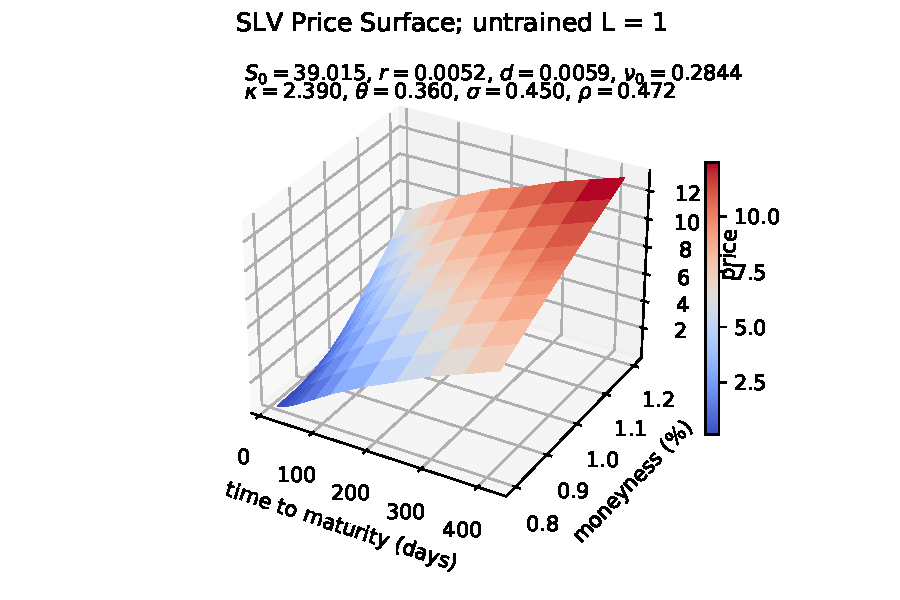
\includegraphics[width=\textwidth]{fig/Psurf_untrained_2017-01-04}
	\end{minipage}
	\begin{minipage}[Ausrichtung]{0.329\textwidth}
		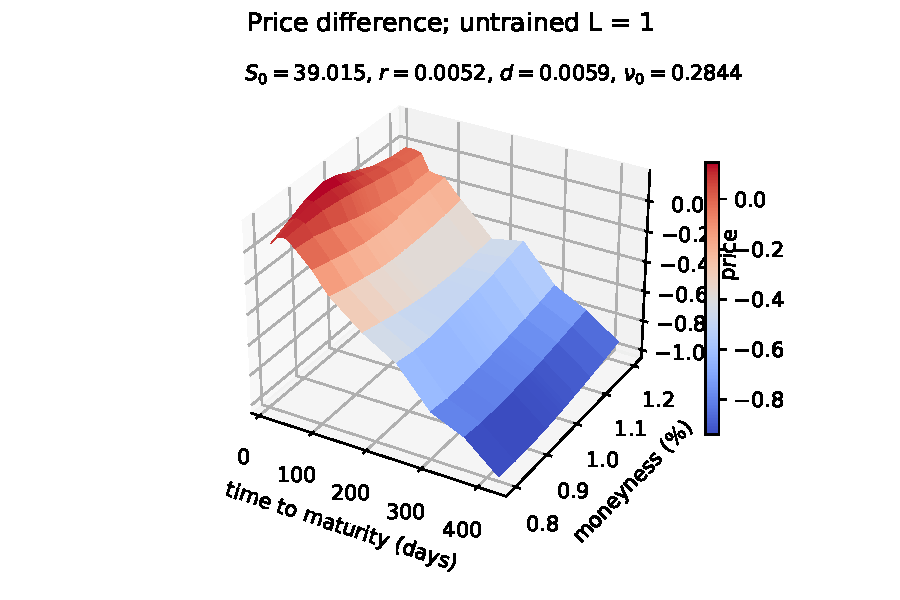
\includegraphics[width=\textwidth]{fig/Psurf_untrained_diff_2017-01-04_rec_3lay_seed1}
	\end{minipage}
	\begin{minipage}[Ausrichtung]{0.329\textwidth}
		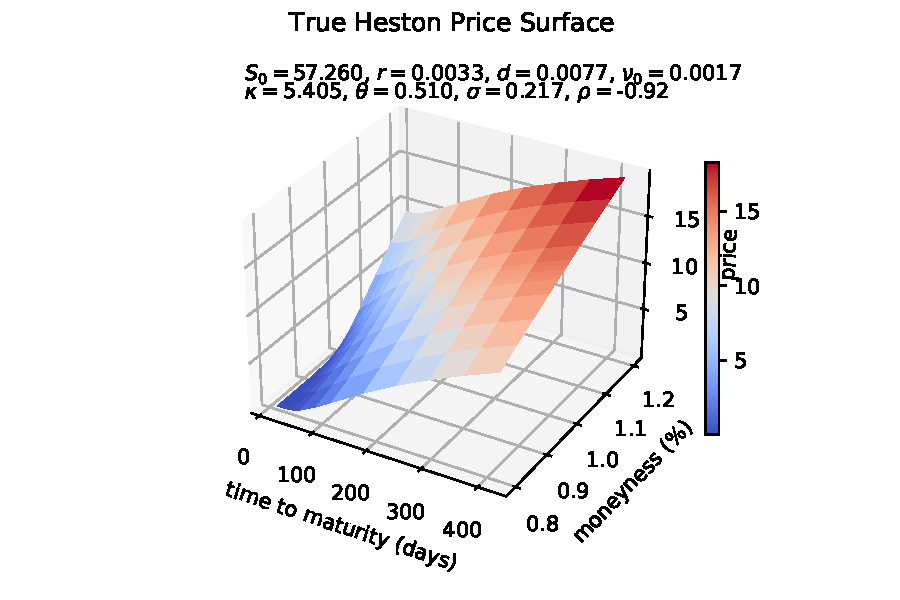
\includegraphics[width=\textwidth]{fig/Psurf_orginal_2017-01-05}
	\end{minipage}
	\begin{minipage}[Ausrichtung]{0.329\textwidth}
		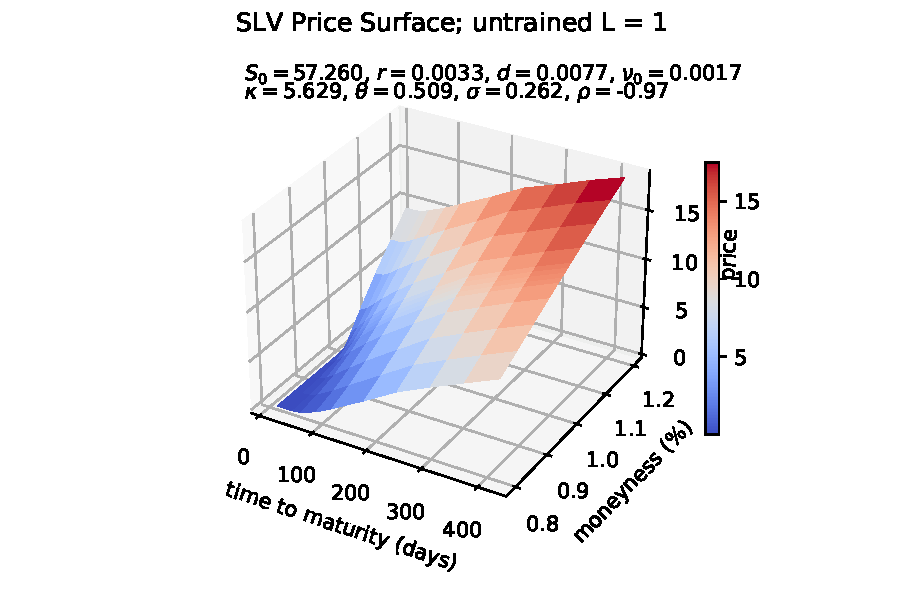
\includegraphics[width=\textwidth]{fig/Psurf_untrained_2017-01-05}
	\end{minipage}
	\begin{minipage}[Ausrichtung]{0.329\textwidth}
		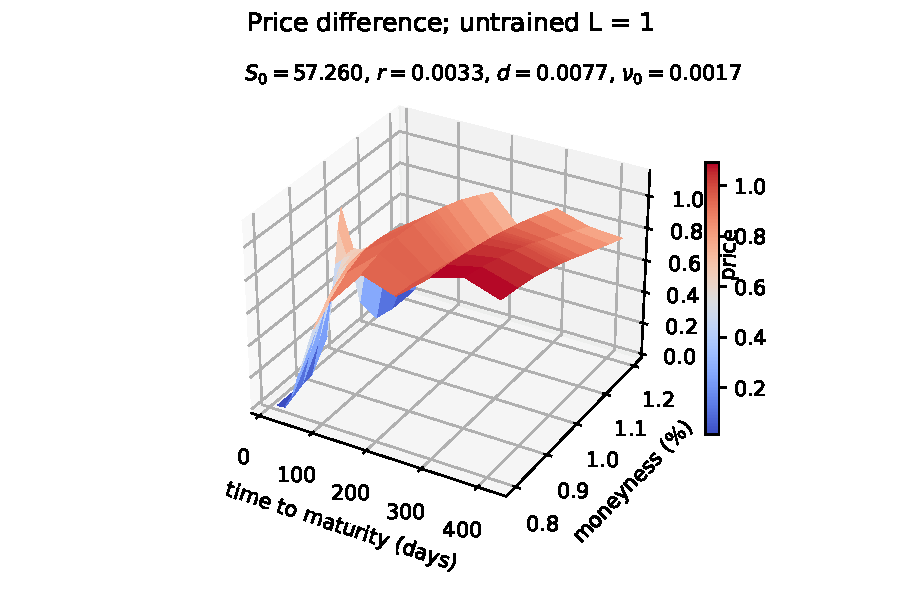
\includegraphics[width=\textwidth]{fig/Psurf_untrained_diff_2017-01-05_rec_3lay_seed1}
	\end{minipage}
	\caption{Comparison of price surfaces for the true parameters against the calibrated Heston parameters from the calibration routine of \texttt{SLV-calib-stochastic.ipynb}. The left column shows the prices generated by the original Heston model. The middle column shows the same prices, but calculated by sampling from the process \eqref{eq:slvhestonmodel} with untrained leverage function $L(t,S_t) = 1$. The deviations are depicted in the right column. The rows correspond to the five different trading days, each defining a separate calibration problem. The surfaces were obtained by averaging over $10^4$ paths, each.}
	\label{fig:pricesurf_comparison_untrained}
\end{figure}


\subsection{Network architecture and training}\label{sec:architecture_rec}


The calibration of the local part of the SLV-model is achieved in a Monte-Carlo like fashion. The stochastic process is discretized by an Euler scheme and paths of the process are drawn via a neural network. This is implemented in \texttt{TensorFlow} by generating a computational graph, taking $S_0,\nu_0$, the starting time $t_0$ and correlated Brownian increments $dW^S_i,dW^\nu_i$ for each time step as input and outputting the price surface across given maturities $T_1,\dots, T_N$ and strikes $K_1, \dots, K_n$ for this single path. Averaging over paths to obtain expectation values will then be achieved through relatively large batch-sizes.

We assume a total time interval of 420 days. We discretize this time-interval by 28 time-steps, each representing 15 days. The network graph is successively built by calculating the price-increments
\begin{align}
	S_{i+1} &= S_i + (r - d)S_idt + L(t_i,S_i)\sqrt{\nu_i}S_idW^S_i \\
	\nu_{i+1} &= \nu_i + \kappa(\theta - \nu_i)dt + \sigma \sqrt{\nu_i}dW^\nu_i \\
	dt &= 15\,,\quad i=0,\dots,28 \,,
\end{align}
with initial conditions $S_0,\nu_0$. The leverage function $L(t,S) = 1+\mathcal{N}(t,S)$ is itself modeled via a deep neural networks. The architecture of $\mathcal{N}$ is chosen with two hidden layers, each comprising of ten nodes, using the \texttt{tanh}-activation function. Thus, the complete computational graph (sampling paths from the considered SLV-process) can be viewed as a recurrent neural network, where the sub-model $\mathcal{N}(t,S)$ is \textit{recurrently} called on each time-step. Besides the chosen two-layer network, also three-, respectively four-layer network architectures with more then ten nodes per layer were tested. These, however, did not show significantly improved learning behavior but, naturally, necessitates longer training periods. Therefore, we settled on this simple two-layer architecture.

For each of the five calibration days, we generate an individual network (all of the same architecture as described above) and fit the local volatility part for each day separately. For this we feed the network with initial $S_0,\nu_0,t_0$ and the increments of the correlated Wiener processes $dW_i^S, dW_i^\nu$, which, in turn, outputs the full price surface across strikes and maturities. The loss function is given by the squared $\ell_2$ distance of this surface to the original price surface (to which we want to fit) given as target-data to the network.

The training was performed over 50 epochs, each, with $10^5$ training samples and a batch of size $10^4$ (to obtain reasonable stable price surfaces). The overall calibration time for one day was about one minute seconds, each (precise values are given in Fig. \ref{fig:loss}). Note, that a relatively small sized training data set is sufficient for the here considered calibration problem, since only a rather small network (of order 100 parameters) approximating the leverage function is trained. Training and validation loss are shown in Fig. \ref{fig:loss}. In all cases the validation loss nicely follows the trend of the training loss, indicating that overfitting is no problem for the proposed calibration scheme. One sees, for all days the networks converge to a essentially stable minimum within roughly five to ten epochs, suggesting that a much shorter training is already be sufficient for a reasonable fit of the leverage function. In light of this fast convergence to a stable minimum, the calibration time can be reduced to approximately five to ten seconds for each day (corresponding to five to ten training epochst). A short training time with reasonable performance is pivotal for the usability of this approach in practice, since typically the model fitting to market data must be very fast.
\begin{figure}
	\centering
	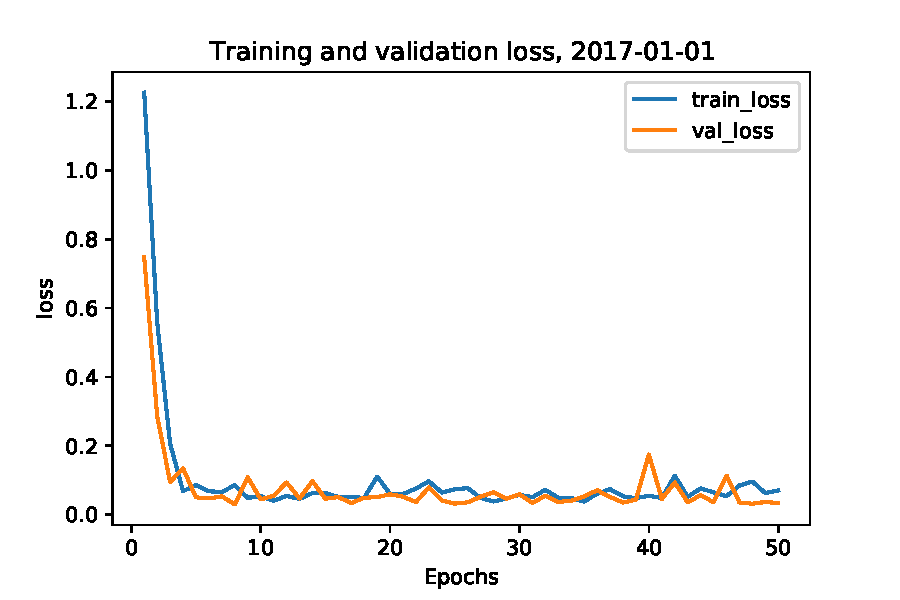
\includegraphics[width=0.32\textwidth]{fig/loss2017-01-01_rec_3lay_seed1.pdf}
	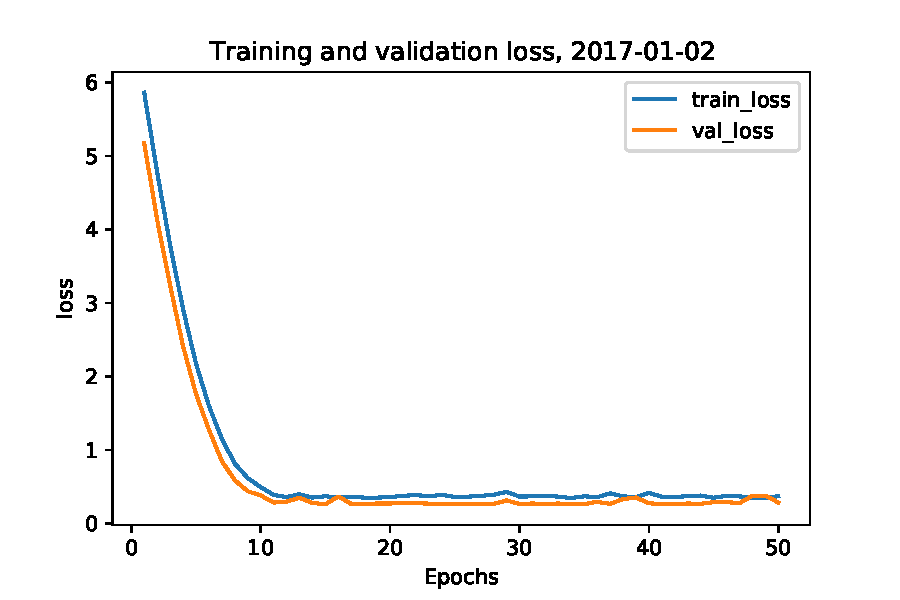
\includegraphics[width=0.32\textwidth]{fig/loss2017-01-02_rec_3lay_seed1.pdf}
	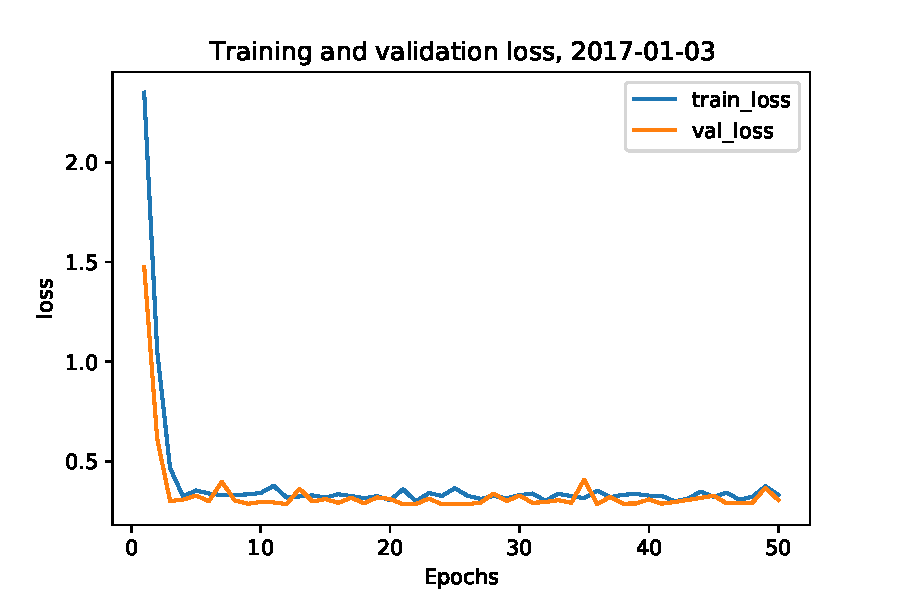
\includegraphics[width=0.32\textwidth]{fig/loss2017-01-03_rec_3lay_seed1.pdf}
	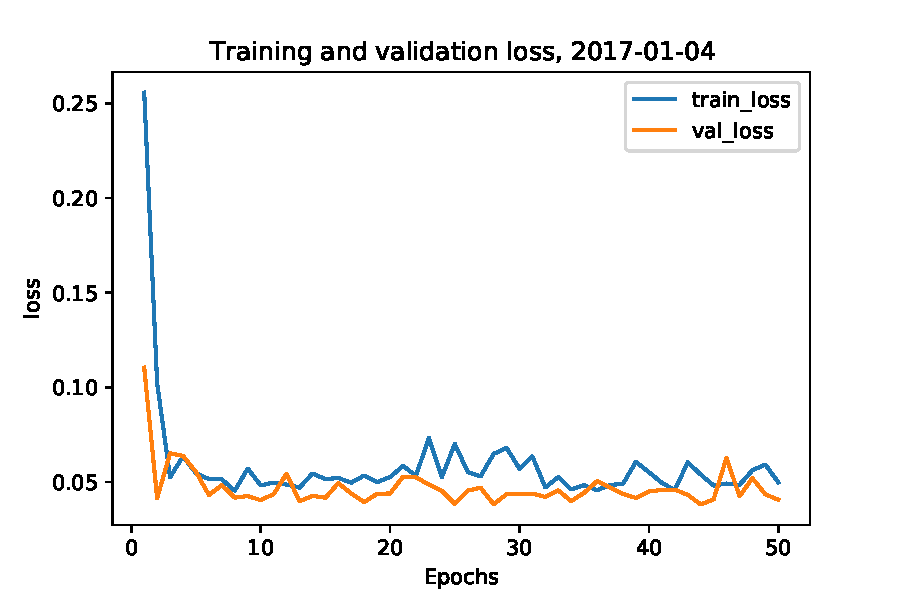
\includegraphics[width=0.32\textwidth]{fig/loss2017-01-04_rec_3lay_seed1.pdf}
	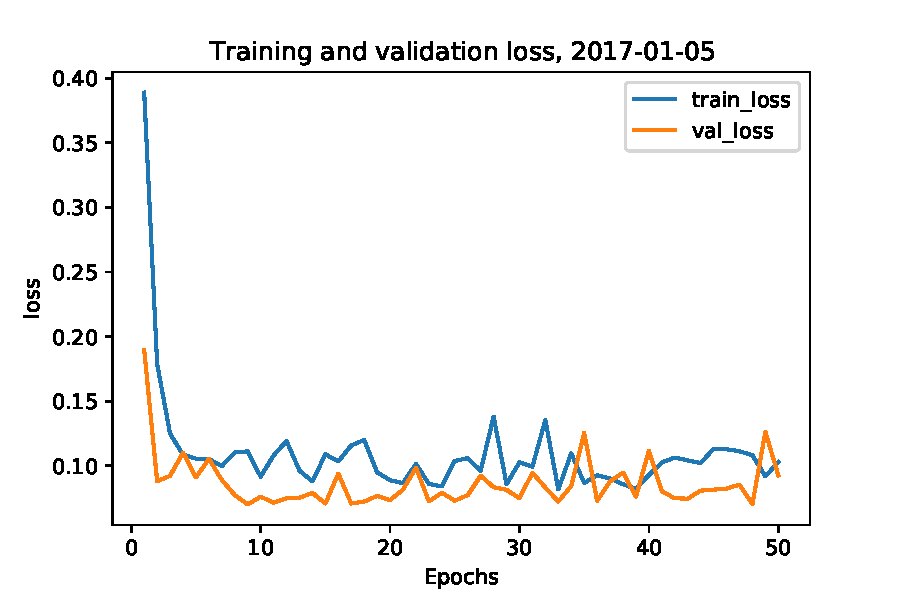
\includegraphics[width=0.32\textwidth]{fig/loss2017-01-05_rec_3lay_seed1.pdf}
	\caption{Training and validation loss during training for 50 epochs of the five networks, each for a specific day. The training times for the five days are $64s, 64s, 65s, 66s, 67s$. As can be seen from the fast convergence of the loss-function, much shorter training intervals of five to ten seconds would be sufficient to achieve the same accuracy in predictions.}
	\label{fig:loss}
\end{figure}

\subsection{Results}

The results of the calibration of the leverage function $L$ are shown in Fig. \ref{fig:pricesurf_comparison_trained}. For compact presentation, only the relevant difference plot between the original price surface (i.e. the target data of the network) and the price surface of the SLV-model after calibration are shown. As one can observe, for all five trading days the discrepancy is reduced by up to  an order of magnitude. This is achieved with a relatively small training data set and short training interval. This suggests that on real market data this combined approach might perform quite well to calibrate the SLV-model \eqref{eq:slvhestonmodel} to observed price, respectively implied volatility data. However, as can be seen from Fig. \ref{fig:pricesurf_comparison_trained}, too, for the second and fifth day at small maturities there are strong peaks in the price surfaces which were nearly unaffected by the training procedure (compare to Fig. \ref{fig:pricesurf_comparison_untrained}). Hence, the neural network seems not able to smoothen out the price surface at small maturities very well. In future studies it would be interesting to see, whether this can be improved upon by adjusting the definition of the loss-function in a way that small maturities are relatively weighted stronger during training.



\begin{figure}
\begin{minipage}{0.49\textwidth}
	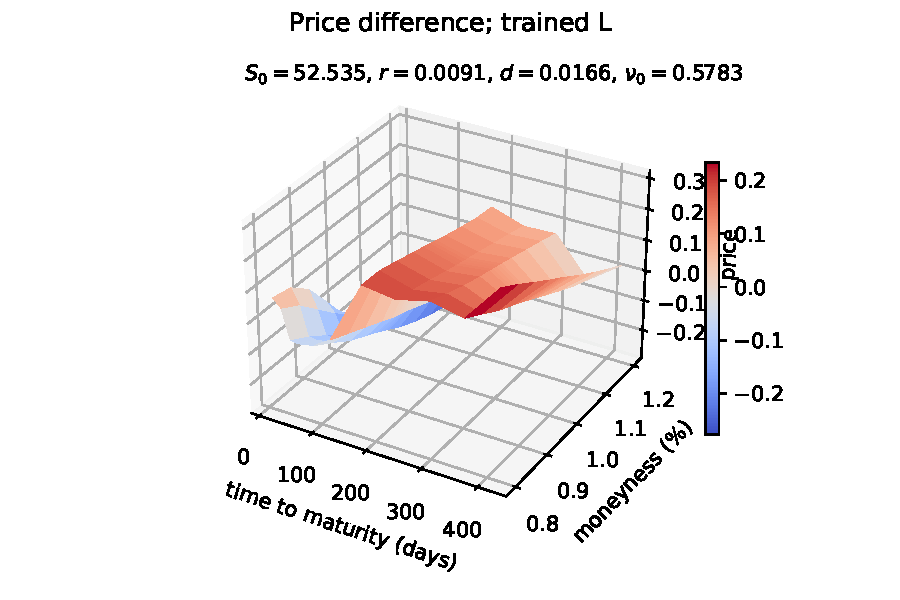
\includegraphics[width=\textwidth]{fig/Psurf_trained_diff_2017-01-01_rec_3lay_seed1}
\end{minipage}
\begin{minipage}{0.49\textwidth}
	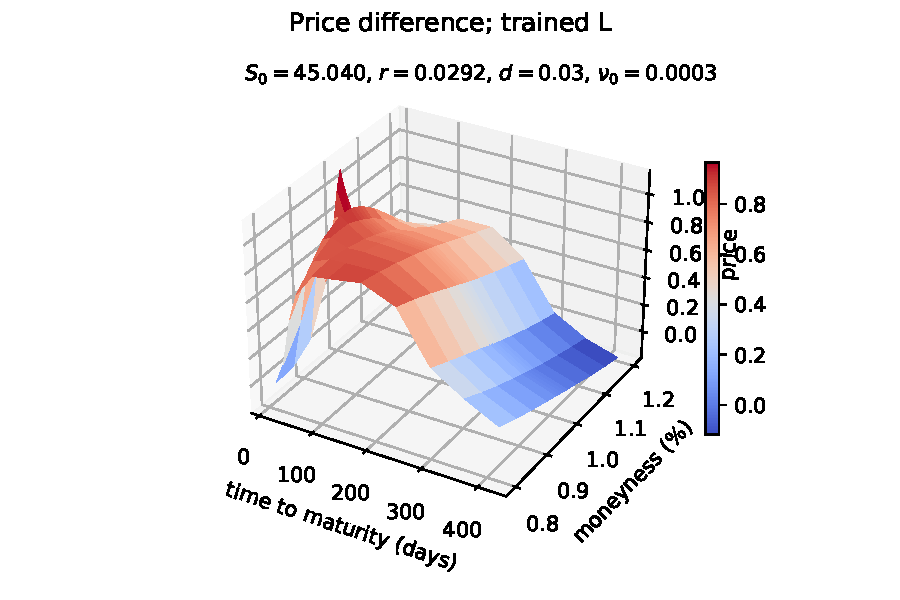
\includegraphics[width=\textwidth]{fig/Psurf_trained_diff_2017-01-02_rec_3lay_seed1}
\end{minipage}
\begin{minipage}{0.49\textwidth}
	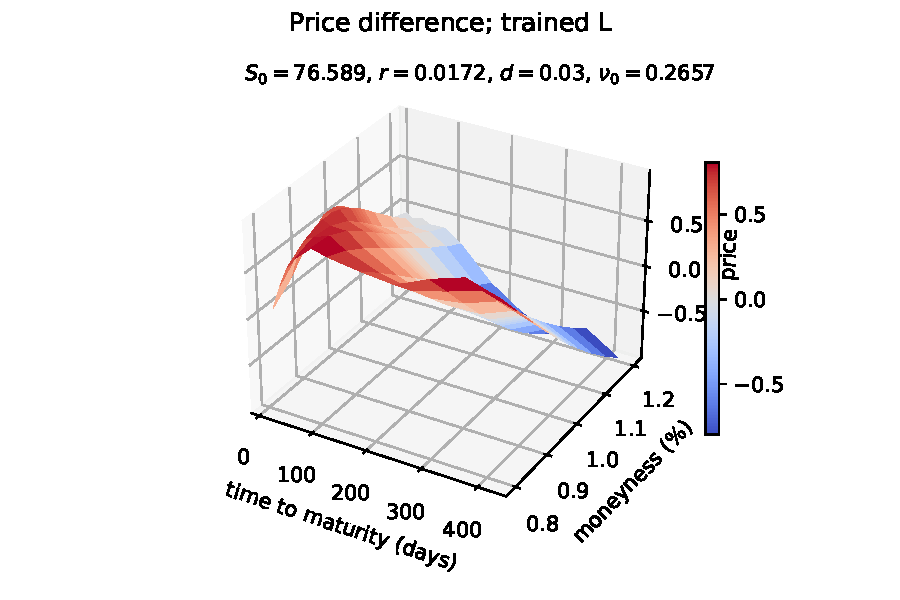
\includegraphics[width=\textwidth]{fig/Psurf_trained_diff_2017-01-03_rec_3lay_seed1}
\end{minipage}
\begin{minipage}{0.49\textwidth}
	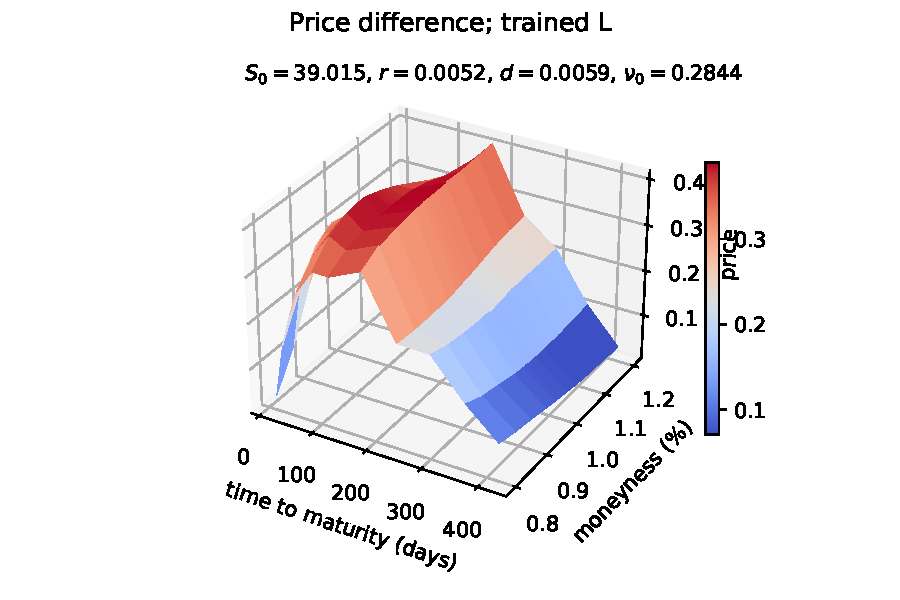
\includegraphics[width=\textwidth]{fig/Psurf_trained_diff_2017-01-04_rec_3lay_seed1}
\end{minipage}
\begin{minipage}{0.49\textwidth}
	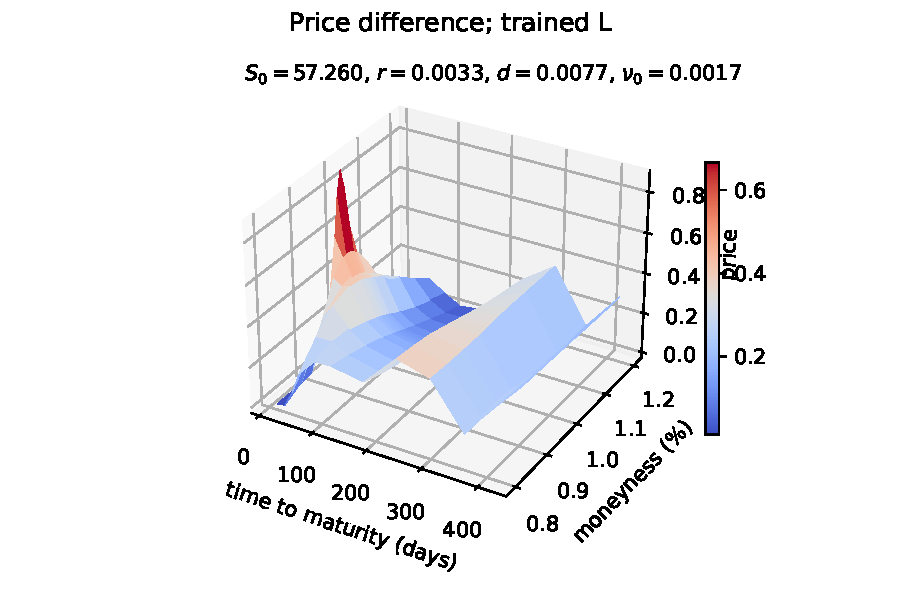
\includegraphics[width=\textwidth]{fig/Psurf_trained_diff_2017-01-05_rec_3lay_seed1}
\end{minipage}
\caption{The plots show the deviations from the original Heston price surface after training. A comparison to the right column of Fig. \ref{fig:pricesurf_comparison_untrained} shows that, for all days, the deviation is reduced by around one order of magnitude. Moreover, the constant shift between both implementations is compensated for and the surfaces are smoothed out. The surfaces were generated from $10^4$ paths, each.}
\label{fig:pricesurf_comparison_trained}
\end{figure}

\subsection{Alternative architecture}
In the previous approach we modeled the leverage function as a two-layer neural network, which is called in each time-step in an recurrent way to generate the paths of the SLV-model. This was found to be the most promising approach. However, also tests of different architectures where performed.

As an example, for comparison the time-dependency of the leverage function was modeled by building a separate small network (each with one hidden layer with ten nodes and \texttt{tanh}-activation) for each time-step $L(t,S) = \mathcal{N}_t(S)$. Such an architecture was originally chosen by Cuchiero, Teichmann et al.\footnote{\url{https://nbviewer.jupyter.org/url/people.math.ethz.ch/~jteichma/lecture_ml_web/local_stoch_vol_calibration.ipynb}} for pricing and hedging in a purely local volatility model. The network was trained on $10^5$ data points with batch-size $10^4$ for 50 epochs. The achieved training and validation loss is depicted in Fig. \ref{fig:alternative_loss}.

\begin{figure}
	\centering
	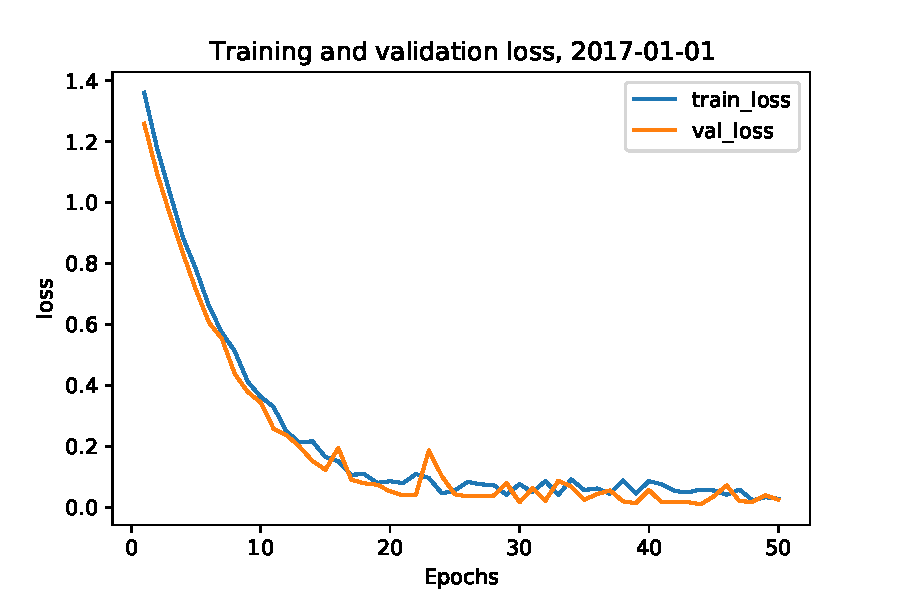
\includegraphics[width=0.32\textwidth]{fig/loss2017-01-01_tnn_seed1.pdf}
	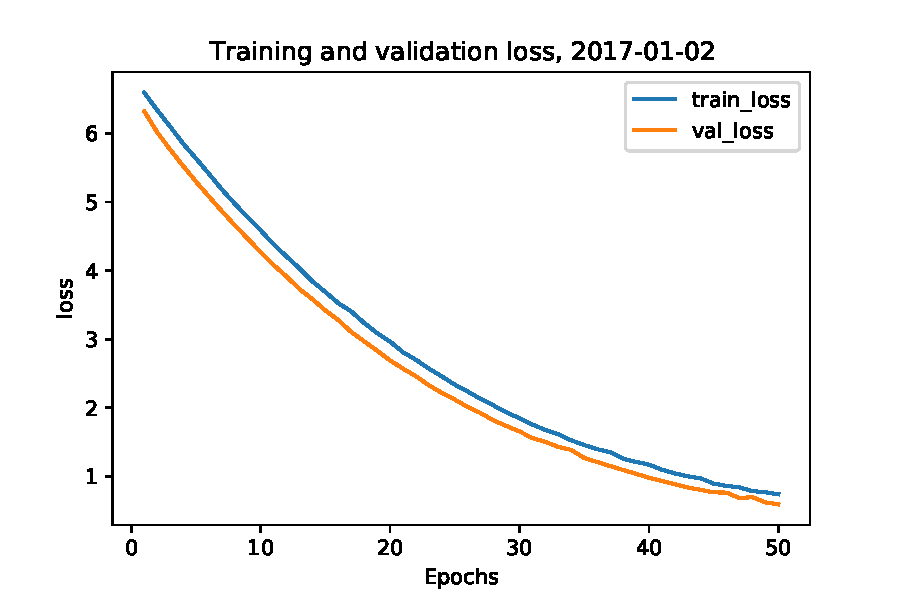
\includegraphics[width=0.32\textwidth]{fig/loss2017-01-02_tnn_seed1.pdf}
	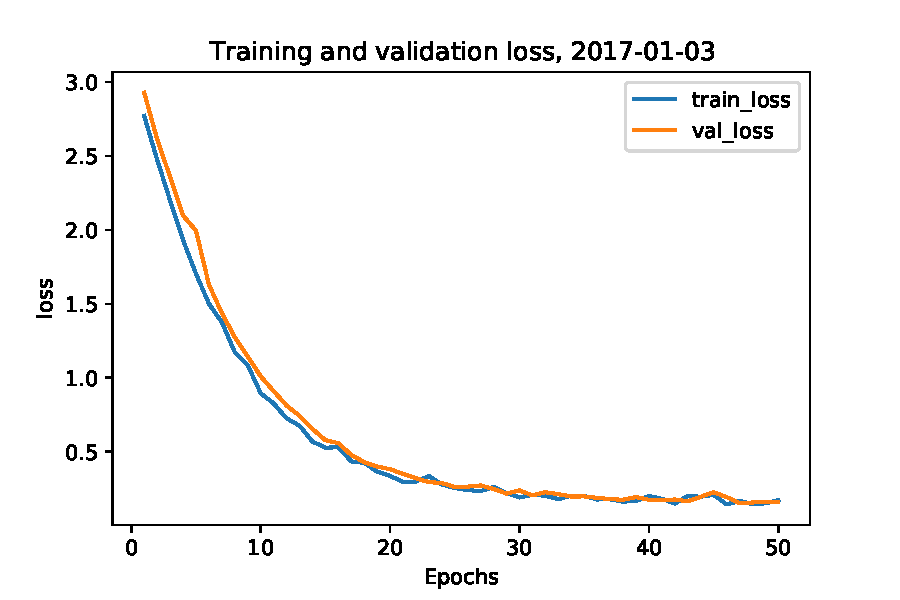
\includegraphics[width=0.32\textwidth]{fig/loss2017-01-03_tnn_seed1.pdf}
	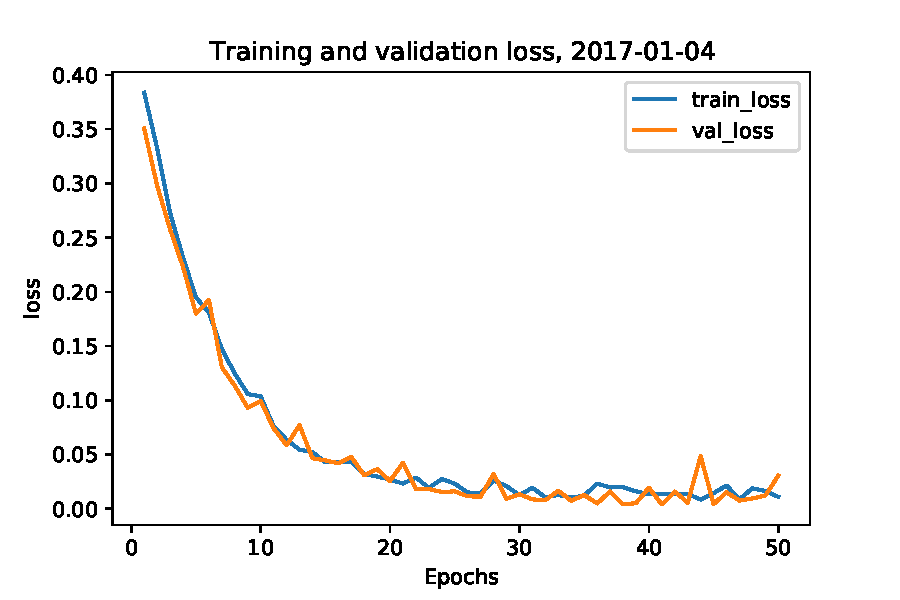
\includegraphics[width=0.32\textwidth]{fig/loss2017-01-04_tnn_seed1.pdf}
	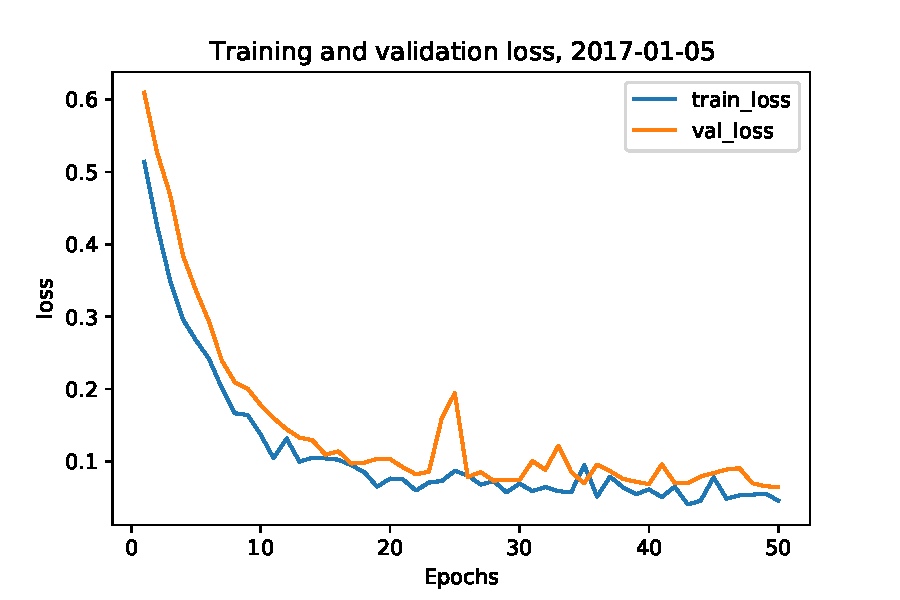
\includegraphics[width=0.32\textwidth]{fig/loss2017-01-05_tnn_seed1.pdf}
	\caption{Training and validation loss during training for 50 epochs of the five networks, each for a specific day. The training times for the five days are $58s, 58s, 59s, 60s, 62s$. The loss-function needs more epochs until convergence as compared to the recurrent network architecture, see Fig. \ref{fig:loss}. However, with the exception of the second day, a comparable accuracy for the predictions is achieved.}
	\label{fig:alternative_loss}
\end{figure}

We see, that in comparison to the recurrent architecture (see Fig. \ref{fig:loss}), the networks achieve similar loss values after training. The exact training times, approximately one minute, each, are given in Fig. \ref{fig:alternative_loss}. Judging from the loss-values, the network achieves similar prediction accuracy as compared to the \textit{recurrent} architecture of Sec. \ref{sec:architecture_rec}. The network needs a little less time for the training of 50 epochs as compared to the \textit{recurrent} architecture, however, necessitate a larger number of epochs to converge. Especially, the second days network stands out, as it does not even converge within 50 epochs to a value smaller then one. On the contrary, the recurrent network (Fig. \ref{fig:loss}) realizes a loss value of order $0.5$ already within the first ten epochs.



\section{Discussion and Outlook}

The discussed numerical simulations show the principal suitability of the proposed neural network approach to the calibration of SLV-models. However, a detailed and systematic analysis of the performance of different network architectures is still lacking would be desirable in future investigations. Fig. \ref{fig:loss} shows that the recurrent leverage function architecture converges to a stable, reasonable fit very fast (already after five to ten epochs). This fast convergence is advantageous for practical applications, however, the fit is not perfect, as also visible from the surface comparison plots in Fig. \ref{fig:pricesurf_comparison_trained}. Moreover, as already mentioned in Sec. \ref{sec:architecture_rec}, even with a more complex network architecture of more then two hidden layers for modeling of the leverage function, the network seems not able to learn a significantly better fit than the chosen simple two-layer architecture. Further testing of alternative architectures is needed to gauge whether improved calibration results of the SLV-model are feasible via the presented neural network approach. Also a detailed study of how more elaborate loss-functions, which for example give larger relative weight to small maturities, influence the performance of the proposed networks calibration scheme. For future investigations it is, furthermore, of pivotal importance how the presented approach performs on actual market data and to compare it to already existing approaches for the SLV-model calibration, as e.g. \cite{cozma_calibration_2019,guo_calibration_2019,saporito_calibration_2017}.

There are many other neural networks based approaches which could be facilitated for the discussed calibration problem and which could be studied in future research: A first approach for the SLV calibration would be to directly learn the mapping from the Dupire local volatility surface $\sigma_\text{loc}$ and Heston parameters to the leverage function surface $L(t_i,S_j)$ through a neural network. The training data could be provided by solving the implicit equation \eqref{eq:impliciteq} for known $\sigma_\text{loc}$ and parameter combinations by means of standard methods (which are e.g. provided by the \texttt{QuantLib} library). This is similar in spirit to the direct calibration method developed in \cite{hernandez_model_2016} for the calibration of purely stochastic volatility models. Another option would be to directly tackle the inverse problem \eqref{eq:impliciteq}, by methods of machine learning. Inverse problems are of major importance in many fields from natural science to finance and, henceforth, many attempts where made to approach such problems by neural networks, see e.g. \cite{li_nett_2020,arridge_solving_2019,genzel_solving_2020}. It would be interesting to investigate in which way such methods could be applied to the here studies problem of calibration in stochastic local volatility models.

Another interesting path would be in the direction of transfer learning: In the current studies, each trading day was calibrated in a separate calibration routine. For the second calibration step, i.e. the learning of the leverage function, this was accomplished by building a individual network for each day. It would be interesting to see, whether the pre-trained network weights of, say, day one, can be utilized as ``starting point'' for the calibration of subsequent days. Such a ``warm start'' has the potential to speed up the calibration of the leverage function considerably.



\newpage
\bibliographystyle{amsalpha}
\bibliography{deep_calibration.bib}



\end{document}
